\pagebreak
\section*{Tydzień 2}
Portrety fazowe systemów liniowych\\
\\
Ciągły system dynamiczny jest asymptotycznie stabilny, gdy części rzeczywiste jego wartości własnych są  ujemne.\\
Ciągły system dynamiczny jest stabilny, gdy części rzeczywiste jego wartości własnych są  niedodatnie oraz klatki Jordana macierzy $J$ odpowiadające wartością własnym macierzy $A$ położonym na osi urojonej mają wymiary $1\times 1$.
\subsection*{Portrety fazowe}
\textbf{1. Wyznaczyć wielomian charakterystyczny macierzy A i wartości własne}\\
\textbf{2. Wyznaczyć wektory własne macierzy A i narysować je w układzie współrzędnych}\\
Jeśli wektor własny jest związany z $\lambda<0$ to wzdłuż tego wektora trajektorie schodzą do zera.\\
Jeśli z $\lambda>0$, uciekają w nieskończoność\\
\textbf{3. Sprawdzić kierunek trajektorii}\\
Wybieramy punkt np $(1,0)$. Mnożymy macierz A przez ten punkt. Otrzymujemy wektor, który wskazuje kierunek z tego punktu.
\begin{figure}[!h]
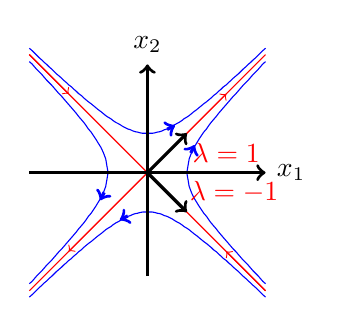
\begin{tikzpicture}[scale=0.5]

\draw [color=blue](-3.0,2.82)--(-2.93,2.76)--(-2.87,2.69)--(-2.81,2.62)--(-2.75,2.56)--(-2.68,2.49)--(-2.62,2.42)--(-2.56,2.35)--(-2.5,2.29)--(-2.43,2.22)--(-2.37,2.15)--(-2.31,2.08)--(-2.25,2.01)--(-2.18,1.94)--(-2.12,1.87)--(-2.06,1.8)--(-2.0,1.73)--(-1.93,1.65)--(-1.87,1.58)--(-1.81,1.51)--(-1.75,1.43)--(-1.68,1.35)--(-1.62,1.28)--(-1.56,1.2)--(-1.5,1.11)--(-1.43,1.03)--(-1.37,0.94)--(-1.31,0.85)--(-1.25,0.75)--(-1.18,0.64)--(-1.12,0.51)--(-1.06,0.35)--(-1.0,0.0)--(-0.93,0.0)--(-0.87,0.0)--(-0.81,0.0)--(-0.75,0.0)--(-0.68,0.0)--(-0.62,0.0)--(-0.56,0.0)--(-0.5,0.0)--(-0.43,0.0)--(-0.37,0.0)--(-0.31,0.0)--(-0.25,0.0)--(-0.18,0.0)--(-0.12,0.0)--(-0.06,0.0)--(0.0,0.0)--(0.06,0.0)--(0.12,0.0)--(0.18,0.0)--(0.25,0.0)--(0.31,0.0)--(0.37,0.0)--(0.43,0.0)--(0.5,0.0)--(0.56,0.0)--(0.62,0.0)--(0.68,0.0)--(0.75,0.0)--(0.81,0.0)--(0.87,0.0)--(0.93,0.0)--(1.0,0.0)--(1.06,0.35)--(1.12,0.51)--(1.18,0.64)--(1.25,0.75)--(1.31,0.85)--(1.37,0.94)--(1.43,1.03)--(1.5,1.11)--(1.56,1.2)--(1.62,1.28)--(1.68,1.35)--(1.75,1.43)--(1.81,1.51)--(1.87,1.58)--(1.93,1.65)--(2.0,1.73)--(2.06,1.8)--(2.12,1.87)--(2.18,1.94)--(2.25,2.01)--(2.31,2.08)--(2.37,2.15)--(2.43,2.22)--(2.5,2.29)--(2.56,2.35)--(2.62,2.42)--(2.68,2.49)--(2.75,2.56)--(2.81,2.62)--(2.87,2.69)--(2.93,2.76)--(3.0,2.82);
\draw [color=blue](-3.0,-2.82)--(-2.93,-2.76)--(-2.87,-2.69)--(-2.81,-2.62)--(-2.75,-2.56)--(-2.68,-2.49)--(-2.62,-2.42)--(-2.56,-2.35)--(-2.5,-2.29)--(-2.43,-2.22)--(-2.37,-2.15)--(-2.31,-2.08)--(-2.25,-2.01)--(-2.18,-1.94)--(-2.12,-1.87)--(-2.06,-1.8)--(-2.0,-1.73)--(-1.93,-1.65)--(-1.87,-1.58)--(-1.81,-1.51)--(-1.75,-1.43)--(-1.68,-1.35)--(-1.62,-1.28)--(-1.56,-1.2)--(-1.5,-1.11)--(-1.43,-1.03)--(-1.37,-0.94)--(-1.31,-0.85)--(-1.25,-0.75)--(-1.18,-0.64)--(-1.12,-0.51)--(-1.06,-0.35)--(-1.0,0.0)--(-0.93,0.0)--(-0.87,0.0)--(-0.81,0.0)--(-0.75,0.0)--(-0.68,0.0)--(-0.62,0.0)--(-0.56,0.0)--(-0.5,0.0)--(-0.43,0.0)--(-0.37,0.0)--(-0.31,0.0)--(-0.25,0.0)--(-0.18,0.0)--(-0.12,0.0)--(-0.06,0.0)--(0.0,0.0)--(0.06,0.0)--(0.12,0.0)--(0.18,0.0)--(0.25,0.0)--(0.31,0.0)--(0.37,0.0)--(0.43,0.0)--(0.5,0.0)--(0.56,0.0)--(0.62,0.0)--(0.68,0.0)--(0.75,0.0)--(0.81,0.0)--(0.87,0.0)--(0.93,0.0)--(1.0,0.0)--(1.06,-0.35)--(1.12,-0.51)--(1.18,-0.64)--(1.25,-0.75)--(1.31,-0.85)--(1.37,-0.94)--(1.43,-1.03)--(1.5,-1.11)--(1.56,-1.2)--(1.62,-1.28)--(1.68,-1.35)--(1.75,-1.43)--(1.81,-1.51)--(1.87,-1.58)--(1.93,-1.65)--(2.0,-1.73)--(2.06,-1.8)--(2.12,-1.87)--(2.18,-1.94)--(2.25,-2.01)--(2.31,-2.08)--(2.37,-2.15)--(2.43,-2.22)--(2.5,-2.29)--(2.56,-2.35)--(2.62,-2.42)--(2.68,-2.49)--(2.75,-2.56)--(2.81,-2.62)--(2.87,-2.69)--(2.93,-2.76)--(3.0,-2.82);
\draw [color=blue](-3.0,3.16)--(-2.93,3.1)--(-2.87,3.04)--(-2.81,2.98)--(-2.75,2.92)--(-2.68,2.86)--(-2.62,2.8)--(-2.56,2.75)--(-2.5,2.69)--(-2.43,2.63)--(-2.37,2.57)--(-2.31,2.51)--(-2.25,2.46)--(-2.18,2.4)--(-2.12,2.34)--(-2.06,2.29)--(-2.0,2.23)--(-1.93,2.18)--(-1.87,2.12)--(-1.81,2.07)--(-1.75,2.01)--(-1.68,1.96)--(-1.62,1.9)--(-1.56,1.85)--(-1.5,1.8)--(-1.43,1.75)--(-1.37,1.7)--(-1.31,1.65)--(-1.25,1.6)--(-1.18,1.55)--(-1.12,1.5)--(-1.06,1.45)--(-1.0,1.41)--(-0.93,1.37)--(-0.87,1.32)--(-0.81,1.28)--(-0.75,1.25)--(-0.68,1.21)--(-0.62,1.17)--(-0.56,1.14)--(-0.5,1.11)--(-0.43,1.09)--(-0.37,1.06)--(-0.31,1.04)--(-0.25,1.03)--(-0.18,1.01)--(-0.12,1.0)--(-0.06,1.0)--(0.0,1.0)--(0.06,1.0)--(0.12,1.0)--(0.18,1.01)--(0.25,1.03)--(0.31,1.04)--(0.37,1.06)--(0.43,1.09)--(0.5,1.11)--(0.56,1.14)--(0.62,1.17)--(0.68,1.21)--(0.75,1.25)--(0.81,1.28)--(0.87,1.32)--(0.93,1.37)--(1.0,1.41)--(1.06,1.45)--(1.12,1.5)--(1.18,1.55)--(1.25,1.6)--(1.31,1.65)--(1.37,1.7)--(1.43,1.75)--(1.5,1.8)--(1.56,1.85)--(1.62,1.9)--(1.68,1.96)--(1.75,2.01)--(1.81,2.07)--(1.87,2.12)--(1.93,2.18)--(2.0,2.23)--(2.06,2.29)--(2.12,2.34)--(2.18,2.4)--(2.25,2.46)--(2.31,2.51)--(2.37,2.57)--(2.43,2.63)--(2.5,2.69)--(2.56,2.75)--(2.62,2.8)--(2.68,2.86)--(2.75,2.92)--(2.81,2.98)--(2.87,3.04)--(2.93,3.1)--(3.0,3.16);
\draw [color=blue](-3.0,-3.16)--(-2.93,-3.1)--(-2.87,-3.04)--(-2.81,-2.98)--(-2.75,-2.92)--(-2.68,-2.86)--(-2.62,-2.8)--(-2.56,-2.75)--(-2.5,-2.69)--(-2.43,-2.63)--(-2.37,-2.57)--(-2.31,-2.51)--(-2.25,-2.46)--(-2.18,-2.4)--(-2.12,-2.34)--(-2.06,-2.29)--(-2.0,-2.23)--(-1.93,-2.18)--(-1.87,-2.12)--(-1.81,-2.07)--(-1.75,-2.01)--(-1.68,-1.96)--(-1.62,-1.9)--(-1.56,-1.85)--(-1.5,-1.8)--(-1.43,-1.75)--(-1.37,-1.7)--(-1.31,-1.65)--(-1.25,-1.6)--(-1.18,-1.55)--(-1.12,-1.5)--(-1.06,-1.45)--(-1.0,-1.41)--(-0.93,-1.37)--(-0.87,-1.32)--(-0.81,-1.28)--(-0.75,-1.25)--(-0.68,-1.21)--(-0.62,-1.17)--(-0.56,-1.14)--(-0.5,-1.11)--(-0.43,-1.09)--(-0.37,-1.06)--(-0.31,-1.04)--(-0.25,-1.03)--(-0.18,-1.01)--(-0.12,-1.0)--(-0.06,-1.0)--(0.0,-1.0)--(0.06,-1.0)--(0.12,-1.0)--(0.18,-1.01)--(0.25,-1.03)--(0.31,-1.04)--(0.37,-1.06)--(0.43,-1.09)--(0.5,-1.11)--(0.56,-1.14)--(0.62,-1.17)--(0.68,-1.21)--(0.75,-1.25)--(0.81,-1.28)--(0.87,-1.32)--(0.93,-1.37)--(1.0,-1.41)--(1.06,-1.45)--(1.12,-1.5)--(1.18,-1.55)--(1.25,-1.6)--(1.31,-1.65)--(1.37,-1.7)--(1.43,-1.75)--(1.5,-1.8)--(1.56,-1.85)--(1.62,-1.9)--(1.68,-1.96)--(1.75,-2.01)--(1.81,-2.07)--(1.87,-2.12)--(1.93,-2.18)--(2.0,-2.23)--(2.06,-2.29)--(2.12,-2.34)--(2.18,-2.4)--(2.25,-2.46)--(2.31,-2.51)--(2.37,-2.57)--(2.43,-2.63)--(2.5,-2.69)--(2.56,-2.75)--(2.62,-2.8)--(2.68,-2.86)--(2.75,-2.92)--(2.81,-2.98)--(2.87,-3.04)--(2.93,-3.1)--(3.0,-3.16);


	\draw[color=blue,very thick][<-](-.7,-1.2)--(-.5,-1.1);
	\draw[color=blue,very thick][<-](.7,1.2)--(.5,1.1);
	\draw[color=blue,very thick][<-](1.2,.7)--(1.1,.5);
	\draw[color=blue,very thick][<-](-1.2,-.7)--(-1.1,-.5);


	\draw[color=red](-3,-3)--(3,3);
	\draw[color=red](-3,3)--(3,-3);

	\draw[color=red][->](0,0)--(2,2);
	\draw[color=red][->](0,0)--(-2,-2);
	\draw[color=red][->](-3,3)--(-2,2);
	\draw[color=red][->](3,-3)--(2,-2);

	\draw[very thick][->](0,0)--(1,1);
	\draw[very thick][->](0,0)--(1,-1);

	\node[color=red] at(2,.5){$\lambda=1$};
	\node[color=red] at(2.2,-.5){$\lambda=-1$};

	\draw[very thick][->](-3,0)--(3,0) node[right=.2] {$x_1$};
	\draw[very thick][->](0,-2.625)--(0,2.75) node[above=.2] {$x_2$};
\end{tikzpicture}
\end{figure}
\\
\textbf{Klatki Jordana}\\
$\left[\begin{array}{cc}a&0\\0&b\end{array}\right], \lambda=a,b\ \ \ \ \left[\begin{array}{cc}a&1\\0&a\end{array}\right], \lambda=a \ \ \ \ \left[\begin{array}{cc}a&b\\-b&a\end{array}\right], \lambda=a \pm bi$\\
\\
\\
$\left[\begin{array}{cc}-1&0\\0&-1\end{array}\right]$ gwiazda, $\left[\begin{array}{cc}-1&0\\0&-2\end{array}\right]$ węzeł, $\left[\begin{array}{cc}-1&0\\0&0\end{array}\right]$ poziome, $\left[\begin{array}{cc}-1&1\\0&-1\end{array}\right]$ węzeł zdegenerowany, $\left[\begin{array}{cc}-1&0\\0&1\end{array}\right]$ siodło\\\\
$\left[\begin{array}{cc}-1&1\\-1&-1\end{array}\right]$ ognisko, $\left[\begin{array}{cc}0&1\\-1&0\end{array}\right]$ kółka\\
\\
\textbf{Frobenius}\\
\fbox{\parbox{.5\linewidth}{
$Frobenius_{2 \times 2}=\left[\begin{array}{cc}0&1\\-c_{m-2}&-c_{m-1}\end{array}\right]$\\
$m=2$\\\\
$A=\left[\begin{array}{cc}0&1\\1&0\end{array}\right] =\left[\begin{array}{cc}0&1\\-c_0&-c_1\end{array}\right]$\\
$-c_0=1, \ \ -c_1 = 0, \boxed{\text{zawsze } c_2=1 }$\\
i z tego mamy wielomian charakterystyczny:\\
$c_2\lambda^2+c_1\lambda+c_0=0$\\
tutaj : $\lambda^2-1=0$
}}
\pagebreak\\
\textbf{Dla jakich parametrów system będzie asymptotycznie stabilny}\\
1. Sprawdzamy czy macierz jest w postaci Frobeniusa\\
2. Jeśli nie wyliczamy wielomian charakterystyczny ($|A-\lambda I|=0$)\\
3. Na podstawie charakterystycznego tworzymy macierz Hurwitza\\
4. Jeżeli wszystkie minory są większe od 0 to system jest asymptotycznie stabilny\\
5. Jeżeli jeden minor jest równy 0 to system jest stabilny, przeciwnie niestabilny\\
\\
\textbf{Zbadaj charakter pracy układu w zależności od parametrów}\\
1. Podstawiamy $u(t)$ do pierwszego równania\\
2. Grupujemy współczynniki\\
3. Tworzymy wielomian charakterystyczny\\
4. Tworzymy macierz Hurwitza\\
5. Sprawdzamy czy minory są większe od 0\\
6. Rysujemy wykres i zaznaczamy obszary stabilności. Wewnątrz obszaru system jest \textbf{asymptotycznie stabilny}, na prostych granicznych jest \textbf{stabilny}, na przecięciach i w pozostałych obszarach jest \textbf{niestabilny}\\
7. Delta wielomianu charakterystycznego <0\\
8. Obliczamy nierówność kwadratową w zależności od $k_2$\\
9. Rysujemy tą funkcję\\
10. Powyżej funkcji będą występować oscylacje, poniżej zanikanie wykładnicze\\
\\
\textbf{Liczenie $e^{At}$}\\
1. równanie charakterystyczne\\
2. Wektory własne\\
3. Macierze $P$, $P^{-1}$, $J$\\
4. $e^{Jt}=e^\lambda \cdot J$\\
5. $e^{At}=P\cdot e^{Jt}\cdot P^{-1}$\\

\pagebreak
%###################                 2.1.1              #################################%
\subsection*{Zadanie 2.1.1} {\color{darkgray}
	Naszkicować portrety fazowe systemów dynamicznych\\
	$\dot{x}(t)=\left[\begin{array}{cc}0&1\\-1&0\end{array}\right]x(t)\ \ \ $ i $\ \ \ \dot{x}(t)=\left[\begin{array}{cc}0&1\\1&0\end{array}\right]x(t)$\\
	i opisać czym się różnią.\\
}\lineh
\\\\
\begin{multicols}{2}\noindent
$\lambda^2+1=0$\\
$\lambda = \pm i$\\
$J=A$\\
$\left[\begin{array}{cc}-i&1\\-1&-i\end{array}\right]\left[\begin{array}{c}\omega_1\\ \omega_2\end{array}\right]=\left[\begin{array}{c}0\\0\end{array}\right]$\\
$-i\omega_1+\omega_2 =0$\\
$-\omega_1-i\omega_2=0$\\
$\omega_1=-i\omega_2$
\\\\\\\\\\\\\\\\\\\\\\\\\\\\\\\\\\
$\lambda^2=1$\\
$\lambda = \pm 1$\\
$J=\left[\begin{array}{cc}\lambda_1&0\\0&\lambda_2\end{array}\right]=\left[\begin{array}{cc}1&0\\0&-1\end{array}\right] \neq A$\\
$\boxed{\lambda=1}$\\
$\left[\begin{array}{cc}-1&1\\1&-1\end{array}\right]\left[\begin{array}{c}\omega_1\\ \omega_2\end{array}\right]=\left[\begin{array}{c}0\\0\end{array}\right]$\\
$ \begin{cases} -\omega_1+\omega_2 =0\\ \omega_1-\omega_2=0\\\end{cases}\Rightarrow \omega_1=\omega_2$\\
$\boxed{\lambda=-1}$\\
$\left[\begin{array}{cc}1&1\\1&1\end{array}\right]\left[\begin{array}{c}\omega_1\\ \omega_2\end{array}\right]=\left[\begin{array}{c}0\\0\end{array}\right]$\\
$ \omega_1+\omega_2 = 0\Rightarrow \omega_1=-\omega_2$\\
\\
wektory własne:\\
$\left[\begin{array}{c}1\\1\end{array}\right] \wedge \left[\begin{array}{c}-1\\1\end{array}\right] \ $ wyznaczają osie\\\\
kierunek strzałek:\\
$\left[\begin{array}{cc}0&1\\1&0\end{array}\right]\left[\begin{array}{c}1\\1\end{array}\right]=\left[\begin{array}{c}1\\1\end{array}\right]$ taki sam wektor więc strzałki $+\infty \ \ -\infty$\\\\
$\left[\begin{array}{cc}0&1\\1&0\end{array}\right]\left[\begin{array}{c}-1\\1\end{array}\right]=\left[\begin{array}{c}1\\-1\end{array}\right]$ inny więc strzałki do 0\\

\end{multicols}
\begin{figure}[!h]
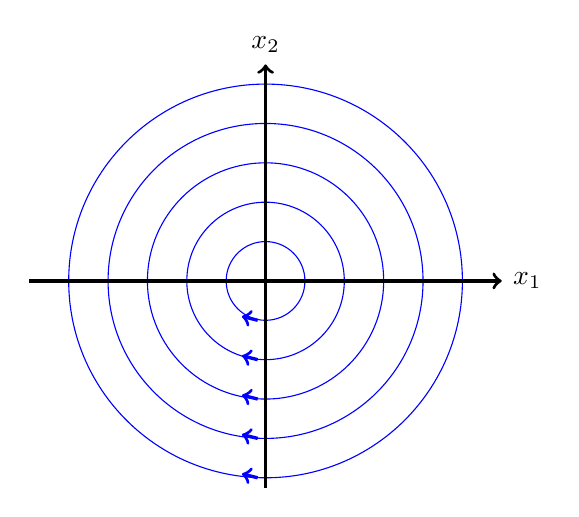
\begin{tikzpicture}
	\draw[color=blue] (0,0) circle(.5);
	\draw[color=blue] (0,0) circle(1);
	\draw[color=blue] (0,0) circle(1.5);
	\draw[color=blue] (0,0) circle(2);
	\draw[color=blue] (0,0) circle(2.5);

	\draw[color=blue,very thick][<-](-.3,-.45)--(-.1,-.5);
	\draw[color=blue,very thick][<-](-.3,-.95)--(-.1,-1);
	\draw[color=blue,very thick][<-](-.3,-1.45)--(-.1,-1.5);
	\draw[color=blue,very thick][<-](-.3,-1.95)--(-.1,-2);
	\draw[color=blue,very thick][<-](-.3,-2.45)--(-.1,-2.5);

	\draw[very thick][->](-3,0)--(3,0) node[right=.2] {$x_1$};
	\draw[very thick][->](0,-2.625)--(0,2.75) node[above=.2] {$x_2$};
\end{tikzpicture}
\hspace*{3cm}
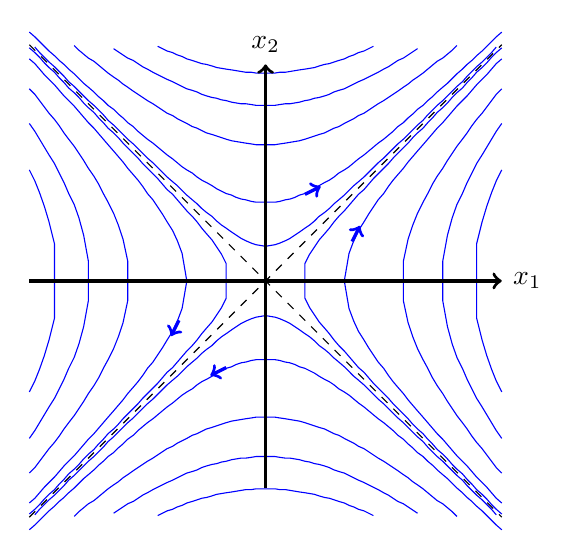
\begin{tikzpicture}
\draw [color=blue](-3.0,2.96)--(-2.93,2.9)--(-2.87,2.84)--(-2.81,2.77)--(-2.75,2.71)--(-2.68,2.65)--(-2.62,2.58)--(-2.56,2.52)--(-2.5,2.45)--(-2.43,2.39)--(-2.37,2.33)--(-2.31,2.26)--(-2.25,2.2)--(-2.18,2.14)--(-2.12,2.07)--(-2.06,2.01)--(-2.0,1.94)--(-1.93,1.88)--(-1.87,1.82)--(-1.81,1.75)--(-1.75,1.69)--(-1.68,1.62)--(-1.62,1.56)--(-1.56,1.49)--(-1.5,1.43)--(-1.43,1.36)--(-1.37,1.3)--(-1.31,1.23)--(-1.25,1.16)--(-1.18,1.1)--(-1.12,1.03)--(-1.06,0.96)--(-1.0,0.89)--(-0.93,0.82)--(-0.87,0.75)--(-0.81,0.67)--(-0.75,0.6)--(-0.68,0.52)--(-0.62,0.43)--(-0.56,0.34)--(-0.5,0.22)--(-0.5,-0.22)--(-0.56,-0.34)--(-0.62,-0.43)--(-0.68,-0.52)--(-0.75,-0.6)--(-0.81,-0.67)--(-0.87,-0.75)--(-0.93,-0.82)--(-1.0,-0.89)--(-1.06,-0.96)--(-1.12,-1.03)--(-1.18,-1.1)--(-1.25,-1.16)--(-1.31,-1.23)--(-1.37,-1.3)--(-1.43,-1.36)--(-1.5,-1.43)--(-1.56,-1.49)--(-1.62,-1.56)--(-1.68,-1.62)--(-1.75,-1.69)--(-1.81,-1.75)--(-1.87,-1.82)--(-1.93,-1.88)--(-2.0,-1.94)--(-2.06,-2.01)--(-2.12,-2.07)--(-2.18,-2.14)--(-2.25,-2.2)--(-2.31,-2.26)--(-2.37,-2.33)--(-2.43,-2.39)--(-2.5,-2.45)--(-2.56,-2.52)--(-2.62,-2.58)--(-2.68,-2.65)--(-2.75,-2.71)--(-2.81,-2.77)--(-2.87,-2.84)--(-2.93,-2.9)--(-3.0,-2.96);
\draw [color=blue](3.0,2.96)--(2.93,2.9)--(2.87,2.84)--(2.81,2.77)--(2.75,2.71)--(2.68,2.65)--(2.62,2.58)--(2.56,2.52)--(2.5,2.45)--(2.43,2.39)--(2.37,2.33)--(2.31,2.26)--(2.25,2.2)--(2.18,2.14)--(2.12,2.07)--(2.06,2.01)--(2.0,1.94)--(1.93,1.88)--(1.87,1.82)--(1.81,1.75)--(1.75,1.69)--(1.68,1.62)--(1.62,1.56)--(1.56,1.49)--(1.5,1.43)--(1.43,1.36)--(1.37,1.3)--(1.31,1.23)--(1.25,1.16)--(1.18,1.1)--(1.12,1.03)--(1.06,0.96)--(1.0,0.89)--(0.93,0.82)--(0.87,0.75)--(0.81,0.67)--(0.75,0.6)--(0.68,0.52)--(0.62,0.43)--(0.56,0.34)--(0.5,0.22)--(0.5,-0.22)--(0.56,-0.34)--(0.62,-0.43)--(0.68,-0.52)--(0.75,-0.6)--(0.81,-0.67)--(0.87,-0.75)--(0.93,-0.82)--(1.0,-0.89)--(1.06,-0.96)--(1.12,-1.03)--(1.18,-1.1)--(1.25,-1.16)--(1.31,-1.23)--(1.37,-1.3)--(1.43,-1.36)--(1.5,-1.43)--(1.56,-1.49)--(1.62,-1.56)--(1.68,-1.62)--(1.75,-1.69)--(1.81,-1.75)--(1.87,-1.82)--(1.93,-1.88)--(2.0,-1.94)--(2.06,-2.01)--(2.12,-2.07)--(2.18,-2.14)--(2.25,-2.2)--(2.31,-2.26)--(2.37,-2.33)--(2.43,-2.39)--(2.5,-2.45)--(2.56,-2.52)--(2.62,-2.58)--(2.68,-2.65)--(2.75,-2.71)--(2.81,-2.77)--(2.87,-2.84)--(2.93,-2.9)--(3.0,-2.96);
\draw [color=blue](-2.93,2.97)--(-2.87,2.9)--(-2.81,2.84)--(-2.75,2.78)--(-2.68,2.72)--(-2.62,2.66)--(-2.56,2.6)--(-2.5,2.53)--(-2.43,2.47)--(-2.37,2.41)--(-2.31,2.35)--(-2.25,2.29)--(-2.18,2.23)--(-2.12,2.17)--(-2.06,2.11)--(-2.0,2.04)--(-1.93,1.98)--(-1.87,1.92)--(-1.81,1.86)--(-1.75,1.8)--(-1.68,1.74)--(-1.62,1.68)--(-1.56,1.62)--(-1.5,1.56)--(-1.43,1.5)--(-1.37,1.44)--(-1.31,1.38)--(-1.25,1.32)--(-1.18,1.26)--(-1.12,1.21)--(-1.06,1.15)--(-1.0,1.09)--(-0.93,1.03)--(-0.87,0.98)--(-0.81,0.92)--(-0.75,0.87)--(-0.68,0.82)--(-0.62,0.76)--(-0.56,0.71)--(-0.5,0.67)--(-0.43,0.62)--(-0.37,0.58)--(-0.31,0.54)--(-0.25,0.51)--(-0.18,0.48)--(-0.12,0.46)--(-0.06,0.45)--(0.0,0.44)--(0.06,0.45)--(0.12,0.46)--(0.18,0.48)--(0.25,0.51)--(0.31,0.54)--(0.37,0.58)--(0.43,0.62)--(0.5,0.67)--(0.56,0.71)--(0.62,0.76)--(0.68,0.82)--(0.75,0.87)--(0.81,0.92)--(0.87,0.98)--(0.93,1.03)--(1.0,1.09)--(1.06,1.15)--(1.12,1.21)--(1.18,1.26)--(1.25,1.32)--(1.31,1.38)--(1.37,1.44)--(1.43,1.5)--(1.5,1.56)--(1.56,1.62)--(1.62,1.68)--(1.68,1.74)--(1.75,1.8)--(1.81,1.86)--(1.87,1.92)--(1.93,1.98)--(2.0,2.04)--(2.06,2.11)--(2.12,2.17)--(2.18,2.23)--(2.25,2.29)--(2.31,2.35)--(2.37,2.41)--(2.43,2.47)--(2.5,2.53)--(2.56,2.6)--(2.62,2.66)--(2.68,2.72)--(2.75,2.78)--(2.81,2.84)--(2.87,2.9)--(2.93,2.97);
\draw [color=blue](-2.93,-2.97)--(-2.87,-2.9)--(-2.81,-2.84)--(-2.75,-2.78)--(-2.68,-2.72)--(-2.62,-2.66)--(-2.56,-2.6)--(-2.5,-2.53)--(-2.43,-2.47)--(-2.37,-2.41)--(-2.31,-2.35)--(-2.25,-2.29)--(-2.18,-2.23)--(-2.12,-2.17)--(-2.06,-2.11)--(-2.0,-2.04)--(-1.93,-1.98)--(-1.87,-1.92)--(-1.81,-1.86)--(-1.75,-1.8)--(-1.68,-1.74)--(-1.62,-1.68)--(-1.56,-1.62)--(-1.5,-1.56)--(-1.43,-1.5)--(-1.37,-1.44)--(-1.31,-1.38)--(-1.25,-1.32)--(-1.18,-1.26)--(-1.12,-1.21)--(-1.06,-1.15)--(-1.0,-1.09)--(-0.93,-1.03)--(-0.87,-0.98)--(-0.81,-0.92)--(-0.75,-0.87)--(-0.68,-0.82)--(-0.62,-0.76)--(-0.56,-0.71)--(-0.5,-0.67)--(-0.43,-0.62)--(-0.37,-0.58)--(-0.31,-0.54)--(-0.25,-0.51)--(-0.18,-0.48)--(-0.12,-0.46)--(-0.06,-0.45)--(0.0,-0.44)--(0.06,-0.45)--(0.12,-0.46)--(0.18,-0.48)--(0.25,-0.51)--(0.31,-0.54)--(0.37,-0.58)--(0.43,-0.62)--(0.5,-0.67)--(0.56,-0.71)--(0.62,-0.76)--(0.68,-0.82)--(0.75,-0.87)--(0.81,-0.92)--(0.87,-0.98)--(0.93,-1.03)--(1.0,-1.09)--(1.06,-1.15)--(1.12,-1.21)--(1.18,-1.26)--(1.25,-1.32)--(1.31,-1.38)--(1.37,-1.44)--(1.43,-1.5)--(1.5,-1.56)--(1.56,-1.62)--(1.62,-1.68)--(1.68,-1.74)--(1.75,-1.8)--(1.81,-1.86)--(1.87,-1.92)--(1.93,-1.98)--(2.0,-2.04)--(2.06,-2.11)--(2.12,-2.17)--(2.18,-2.23)--(2.25,-2.29)--(2.31,-2.35)--(2.37,-2.41)--(2.43,-2.47)--(2.5,-2.53)--(2.56,-2.6)--(2.62,-2.66)--(2.68,-2.72)--(2.75,-2.78)--(2.81,-2.84)--(2.87,-2.9)--(2.93,-2.97);

\draw [color=blue](-3.0,2.82)--(-2.93,2.76)--(-2.87,2.69)--(-2.81,2.62)--(-2.75,2.56)--(-2.68,2.49)--(-2.62,2.42)--(-2.56,2.35)--(-2.5,2.29)--(-2.43,2.22)--(-2.37,2.15)--(-2.31,2.08)--(-2.25,2.01)--(-2.18,1.94)--(-2.12,1.87)--(-2.06,1.8)--(-2.0,1.73)--(-1.93,1.65)--(-1.87,1.58)--(-1.81,1.51)--(-1.75,1.43)--(-1.68,1.35)--(-1.62,1.28)--(-1.56,1.2)--(-1.5,1.11)--(-1.43,1.03)--(-1.37,0.94)--(-1.31,0.85)--(-1.25,0.75)--(-1.18,0.64)--(-1.12,0.51)--(-1.06,0.35)--(-1.0,0.0)--(-0.93,0.0)--(-0.87,0.0)--(-0.81,0.0)--(-0.75,0.0)--(-0.68,0.0)--(-0.62,0.0)--(-0.56,0.0)--(-0.5,0.0)--(-0.43,0.0)--(-0.37,0.0)--(-0.31,0.0)--(-0.25,0.0)--(-0.18,0.0)--(-0.12,0.0)--(-0.06,0.0)--(0.0,0.0)--(0.06,0.0)--(0.12,0.0)--(0.18,0.0)--(0.25,0.0)--(0.31,0.0)--(0.37,0.0)--(0.43,0.0)--(0.5,0.0)--(0.56,0.0)--(0.62,0.0)--(0.68,0.0)--(0.75,0.0)--(0.81,0.0)--(0.87,0.0)--(0.93,0.0)--(1.0,0.0)--(1.06,0.35)--(1.12,0.51)--(1.18,0.64)--(1.25,0.75)--(1.31,0.85)--(1.37,0.94)--(1.43,1.03)--(1.5,1.11)--(1.56,1.2)--(1.62,1.28)--(1.68,1.35)--(1.75,1.43)--(1.81,1.51)--(1.87,1.58)--(1.93,1.65)--(2.0,1.73)--(2.06,1.8)--(2.12,1.87)--(2.18,1.94)--(2.25,2.01)--(2.31,2.08)--(2.37,2.15)--(2.43,2.22)--(2.5,2.29)--(2.56,2.35)--(2.62,2.42)--(2.68,2.49)--(2.75,2.56)--(2.81,2.62)--(2.87,2.69)--(2.93,2.76)--(3.0,2.82);
\draw [color=blue](-3.0,-2.82)--(-2.93,-2.76)--(-2.87,-2.69)--(-2.81,-2.62)--(-2.75,-2.56)--(-2.68,-2.49)--(-2.62,-2.42)--(-2.56,-2.35)--(-2.5,-2.29)--(-2.43,-2.22)--(-2.37,-2.15)--(-2.31,-2.08)--(-2.25,-2.01)--(-2.18,-1.94)--(-2.12,-1.87)--(-2.06,-1.8)--(-2.0,-1.73)--(-1.93,-1.65)--(-1.87,-1.58)--(-1.81,-1.51)--(-1.75,-1.43)--(-1.68,-1.35)--(-1.62,-1.28)--(-1.56,-1.2)--(-1.5,-1.11)--(-1.43,-1.03)--(-1.37,-0.94)--(-1.31,-0.85)--(-1.25,-0.75)--(-1.18,-0.64)--(-1.12,-0.51)--(-1.06,-0.35)--(-1.0,0.0)--(-0.93,0.0)--(-0.87,0.0)--(-0.81,0.0)--(-0.75,0.0)--(-0.68,0.0)--(-0.62,0.0)--(-0.56,0.0)--(-0.5,0.0)--(-0.43,0.0)--(-0.37,0.0)--(-0.31,0.0)--(-0.25,0.0)--(-0.18,0.0)--(-0.12,0.0)--(-0.06,0.0)--(0.0,0.0)--(0.06,0.0)--(0.12,0.0)--(0.18,0.0)--(0.25,0.0)--(0.31,0.0)--(0.37,0.0)--(0.43,0.0)--(0.5,0.0)--(0.56,0.0)--(0.62,0.0)--(0.68,0.0)--(0.75,0.0)--(0.81,0.0)--(0.87,0.0)--(0.93,0.0)--(1.0,0.0)--(1.06,-0.35)--(1.12,-0.51)--(1.18,-0.64)--(1.25,-0.75)--(1.31,-0.85)--(1.37,-0.94)--(1.43,-1.03)--(1.5,-1.11)--(1.56,-1.2)--(1.62,-1.28)--(1.68,-1.35)--(1.75,-1.43)--(1.81,-1.51)--(1.87,-1.58)--(1.93,-1.65)--(2.0,-1.73)--(2.06,-1.8)--(2.12,-1.87)--(2.18,-1.94)--(2.25,-2.01)--(2.31,-2.08)--(2.37,-2.15)--(2.43,-2.22)--(2.5,-2.29)--(2.56,-2.35)--(2.62,-2.42)--(2.68,-2.49)--(2.75,-2.56)--(2.81,-2.62)--(2.87,-2.69)--(2.93,-2.76)--(3.0,-2.82);
\draw [color=blue](-3.0,3.16)--(-2.93,3.1)--(-2.87,3.04)--(-2.81,2.98)--(-2.75,2.92)--(-2.68,2.86)--(-2.62,2.8)--(-2.56,2.75)--(-2.5,2.69)--(-2.43,2.63)--(-2.37,2.57)--(-2.31,2.51)--(-2.25,2.46)--(-2.18,2.4)--(-2.12,2.34)--(-2.06,2.29)--(-2.0,2.23)--(-1.93,2.18)--(-1.87,2.12)--(-1.81,2.07)--(-1.75,2.01)--(-1.68,1.96)--(-1.62,1.9)--(-1.56,1.85)--(-1.5,1.8)--(-1.43,1.75)--(-1.37,1.7)--(-1.31,1.65)--(-1.25,1.6)--(-1.18,1.55)--(-1.12,1.5)--(-1.06,1.45)--(-1.0,1.41)--(-0.93,1.37)--(-0.87,1.32)--(-0.81,1.28)--(-0.75,1.25)--(-0.68,1.21)--(-0.62,1.17)--(-0.56,1.14)--(-0.5,1.11)--(-0.43,1.09)--(-0.37,1.06)--(-0.31,1.04)--(-0.25,1.03)--(-0.18,1.01)--(-0.12,1.0)--(-0.06,1.0)--(0.0,1.0)--(0.06,1.0)--(0.12,1.0)--(0.18,1.01)--(0.25,1.03)--(0.31,1.04)--(0.37,1.06)--(0.43,1.09)--(0.5,1.11)--(0.56,1.14)--(0.62,1.17)--(0.68,1.21)--(0.75,1.25)--(0.81,1.28)--(0.87,1.32)--(0.93,1.37)--(1.0,1.41)--(1.06,1.45)--(1.12,1.5)--(1.18,1.55)--(1.25,1.6)--(1.31,1.65)--(1.37,1.7)--(1.43,1.75)--(1.5,1.8)--(1.56,1.85)--(1.62,1.9)--(1.68,1.96)--(1.75,2.01)--(1.81,2.07)--(1.87,2.12)--(1.93,2.18)--(2.0,2.23)--(2.06,2.29)--(2.12,2.34)--(2.18,2.4)--(2.25,2.46)--(2.31,2.51)--(2.37,2.57)--(2.43,2.63)--(2.5,2.69)--(2.56,2.75)--(2.62,2.8)--(2.68,2.86)--(2.75,2.92)--(2.81,2.98)--(2.87,3.04)--(2.93,3.1)--(3.0,3.16);
\draw [color=blue](-3.0,-3.16)--(-2.93,-3.1)--(-2.87,-3.04)--(-2.81,-2.98)--(-2.75,-2.92)--(-2.68,-2.86)--(-2.62,-2.8)--(-2.56,-2.75)--(-2.5,-2.69)--(-2.43,-2.63)--(-2.37,-2.57)--(-2.31,-2.51)--(-2.25,-2.46)--(-2.18,-2.4)--(-2.12,-2.34)--(-2.06,-2.29)--(-2.0,-2.23)--(-1.93,-2.18)--(-1.87,-2.12)--(-1.81,-2.07)--(-1.75,-2.01)--(-1.68,-1.96)--(-1.62,-1.9)--(-1.56,-1.85)--(-1.5,-1.8)--(-1.43,-1.75)--(-1.37,-1.7)--(-1.31,-1.65)--(-1.25,-1.6)--(-1.18,-1.55)--(-1.12,-1.5)--(-1.06,-1.45)--(-1.0,-1.41)--(-0.93,-1.37)--(-0.87,-1.32)--(-0.81,-1.28)--(-0.75,-1.25)--(-0.68,-1.21)--(-0.62,-1.17)--(-0.56,-1.14)--(-0.5,-1.11)--(-0.43,-1.09)--(-0.37,-1.06)--(-0.31,-1.04)--(-0.25,-1.03)--(-0.18,-1.01)--(-0.12,-1.0)--(-0.06,-1.0)--(0.0,-1.0)--(0.06,-1.0)--(0.12,-1.0)--(0.18,-1.01)--(0.25,-1.03)--(0.31,-1.04)--(0.37,-1.06)--(0.43,-1.09)--(0.5,-1.11)--(0.56,-1.14)--(0.62,-1.17)--(0.68,-1.21)--(0.75,-1.25)--(0.81,-1.28)--(0.87,-1.32)--(0.93,-1.37)--(1.0,-1.41)--(1.06,-1.45)--(1.12,-1.5)--(1.18,-1.55)--(1.25,-1.6)--(1.31,-1.65)--(1.37,-1.7)--(1.43,-1.75)--(1.5,-1.8)--(1.56,-1.85)--(1.62,-1.9)--(1.68,-1.96)--(1.75,-2.01)--(1.81,-2.07)--(1.87,-2.12)--(1.93,-2.18)--(2.0,-2.23)--(2.06,-2.29)--(2.12,-2.34)--(2.18,-2.4)--(2.25,-2.46)--(2.31,-2.51)--(2.37,-2.57)--(2.43,-2.63)--(2.5,-2.69)--(2.56,-2.75)--(2.62,-2.8)--(2.68,-2.86)--(2.75,-2.92)--(2.81,-2.98)--(2.87,-3.04)--(2.93,-3.1)--(3.0,-3.16);

\draw [color=blue](-3.0,2.44)--(-2.93,2.37)--(-2.87,2.29)--(-2.81,2.21)--(-2.75,2.13)--(-2.68,2.05)--(-2.62,1.97)--(-2.56,1.88)--(-2.5,1.8)--(-2.43,1.71)--(-2.37,1.62)--(-2.31,1.53)--(-2.25,1.43)--(-2.18,1.33)--(-2.12,1.23)--(-2.06,1.11)--(-2.0,1.0)--(-1.93,0.86)--(-1.87,0.71)--(-1.81,0.53)--(-1.75,0.25)--(-1.75,-0.25)--(-1.81,-0.53)--(-1.87,-0.71)--(-1.93,-0.86)--(-2.0,-1.0)--(-2.06,-1.11)--(-2.12,-1.23)--(-2.18,-1.33)--(-2.25,-1.43)--(-2.31,-1.53)--(-2.37,-1.62)--(-2.43,-1.71)--(-2.5,-1.8)--(-2.56,-1.88)--(-2.62,-1.97)--(-2.68,-2.05)--(-2.75,-2.13)--(-2.81,-2.21)--(-2.87,-2.29)--(-2.93,-2.37)--(-3.0,-2.44);
\draw [color=blue](3.0,2.44)--(2.93,2.37)--(2.87,2.29)--(2.81,2.21)--(2.75,2.13)--(2.68,2.05)--(2.62,1.97)--(2.56,1.88)--(2.5,1.8)--(2.43,1.71)--(2.37,1.62)--(2.31,1.53)--(2.25,1.43)--(2.18,1.33)--(2.12,1.23)--(2.06,1.11)--(2.0,1.0)--(1.93,0.86)--(1.87,0.71)--(1.81,0.53)--(1.75,0.25)--(1.75,-0.25)--(1.81,-0.53)--(1.87,-0.71)--(1.93,-0.86)--(2.0,-1.0)--(2.06,-1.11)--(2.12,-1.23)--(2.18,-1.33)--(2.25,-1.43)--(2.31,-1.53)--(2.37,-1.62)--(2.43,-1.71)--(2.5,-1.8)--(2.56,-1.88)--(2.62,-1.97)--(2.68,-2.05)--(2.75,-2.13)--(2.81,-2.21)--(2.87,-2.29)--(2.93,-2.37)--(3.0,-2.44);
\draw [color=blue](-2.43,2.99)--(-2.37,2.93)--(-2.31,2.88)--(-2.25,2.83)--(-2.18,2.79)--(-2.12,2.74)--(-2.06,2.69)--(-2.0,2.64)--(-1.93,2.59)--(-1.87,2.55)--(-1.81,2.5)--(-1.75,2.46)--(-1.68,2.41)--(-1.62,2.37)--(-1.56,2.33)--(-1.5,2.29)--(-1.43,2.25)--(-1.37,2.21)--(-1.31,2.17)--(-1.25,2.13)--(-1.18,2.1)--(-1.12,2.06)--(-1.06,2.03)--(-1.0,2.0)--(-0.93,1.96)--(-0.87,1.94)--(-0.81,1.91)--(-0.75,1.88)--(-0.68,1.86)--(-0.62,1.84)--(-0.56,1.82)--(-0.5,1.8)--(-0.43,1.78)--(-0.37,1.77)--(-0.31,1.76)--(-0.25,1.75)--(-0.18,1.74)--(-0.12,1.73)--(-0.06,1.73)--(0.0,1.73)--(0.06,1.73)--(0.12,1.73)--(0.18,1.74)--(0.25,1.75)--(0.31,1.76)--(0.37,1.77)--(0.43,1.78)--(0.5,1.8)--(0.56,1.82)--(0.62,1.84)--(0.68,1.86)--(0.75,1.88)--(0.81,1.91)--(0.87,1.94)--(0.93,1.96)--(1.0,2.0)--(1.06,2.03)--(1.12,2.06)--(1.18,2.1)--(1.25,2.13)--(1.31,2.17)--(1.37,2.21)--(1.43,2.25)--(1.5,2.29)--(1.56,2.33)--(1.62,2.37)--(1.68,2.41)--(1.75,2.46)--(1.81,2.5)--(1.87,2.55)--(1.93,2.59)--(2.0,2.64)--(2.06,2.69)--(2.12,2.74)--(2.18,2.79)--(2.25,2.83)--(2.31,2.88)--(2.37,2.93)--(2.43,2.99);
\draw [color=blue](-2.43,-2.99)--(-2.37,-2.93)--(-2.31,-2.88)--(-2.25,-2.83)--(-2.18,-2.79)--(-2.12,-2.74)--(-2.06,-2.69)--(-2.0,-2.64)--(-1.93,-2.59)--(-1.87,-2.55)--(-1.81,-2.5)--(-1.75,-2.46)--(-1.68,-2.41)--(-1.62,-2.37)--(-1.56,-2.33)--(-1.5,-2.29)--(-1.43,-2.25)--(-1.37,-2.21)--(-1.31,-2.17)--(-1.25,-2.13)--(-1.18,-2.1)--(-1.12,-2.06)--(-1.06,-2.03)--(-1.0,-2.0)--(-0.93,-1.96)--(-0.87,-1.94)--(-0.81,-1.91)--(-0.75,-1.88)--(-0.68,-1.86)--(-0.62,-1.84)--(-0.56,-1.82)--(-0.5,-1.8)--(-0.43,-1.78)--(-0.37,-1.77)--(-0.31,-1.76)--(-0.25,-1.75)--(-0.18,-1.74)--(-0.12,-1.73)--(-0.06,-1.73)--(0.0,-1.73)--(0.06,-1.73)--(0.12,-1.73)--(0.18,-1.74)--(0.25,-1.75)--(0.31,-1.76)--(0.37,-1.77)--(0.43,-1.78)--(0.5,-1.8)--(0.56,-1.82)--(0.62,-1.84)--(0.68,-1.86)--(0.75,-1.88)--(0.81,-1.91)--(0.87,-1.94)--(0.93,-1.96)--(1.0,-2.0)--(1.06,-2.03)--(1.12,-2.06)--(1.18,-2.1)--(1.25,-2.13)--(1.31,-2.17)--(1.37,-2.21)--(1.43,-2.25)--(1.5,-2.29)--(1.56,-2.33)--(1.62,-2.37)--(1.68,-2.41)--(1.75,-2.46)--(1.81,-2.5)--(1.87,-2.55)--(1.93,-2.59)--(2.0,-2.64)--(2.06,-2.69)--(2.12,-2.74)--(2.18,-2.79)--(2.25,-2.83)--(2.31,-2.88)--(2.37,-2.93)--(2.43,-2.99);


\draw [color=blue](-3.0,2.0)--(-2.93,1.9)--(-2.87,1.8)--(-2.81,1.7)--(-2.75,1.6)--(-2.68,1.49)--(-2.62,1.37)--(-2.56,1.25)--(-2.5,1.11)--(-2.43,0.97)--(-2.37,0.8)--(-2.31,0.58)--(-2.25,0.25)--(-2.25,-0.25)--(-2.31,-0.58)--(-2.37,-0.8)--(-2.43,-0.97)--(-2.5,-1.11)--(-2.56,-1.25)--(-2.62,-1.37)--(-2.68,-1.49)--(-2.75,-1.6)--(-2.81,-1.7)--(-2.87,-1.8)--(-2.93,-1.9)--(-3.0,-2.0);
\draw [color=blue](3.0,2.0)--(2.93,1.9)--(2.87,1.8)--(2.81,1.7)--(2.75,1.6)--(2.68,1.49)--(2.62,1.37)--(2.56,1.25)--(2.5,1.11)--(2.43,0.97)--(2.37,0.8)--(2.31,0.58)--(2.25,0.25)--(2.25,-0.25)--(2.31,-0.58)--(2.37,-0.8)--(2.43,-0.97)--(2.5,-1.11)--(2.56,-1.25)--(2.62,-1.37)--(2.68,-1.49)--(2.75,-1.6)--(2.81,-1.7)--(2.87,-1.8)--(2.93,-1.9)--(3.0,-2.0);
\draw [color=blue](-1.93,2.95)--(-1.87,2.91)--(-1.81,2.87)--(-1.75,2.83)--(-1.68,2.8)--(-1.62,2.76)--(-1.56,2.72)--(-1.5,2.69)--(-1.43,2.65)--(-1.37,2.62)--(-1.31,2.59)--(-1.25,2.56)--(-1.18,2.53)--(-1.12,2.5)--(-1.06,2.47)--(-1.0,2.44)--(-0.93,2.42)--(-0.87,2.4)--(-0.81,2.37)--(-0.75,2.35)--(-0.68,2.33)--(-0.62,2.32)--(-0.56,2.3)--(-0.5,2.29)--(-0.43,2.27)--(-0.37,2.26)--(-0.31,2.25)--(-0.25,2.25)--(-0.18,2.24)--(-0.12,2.23)--(-0.06,2.23)--(0.0,2.23)--(0.06,2.23)--(0.12,2.23)--(0.18,2.24)--(0.25,2.25)--(0.31,2.25)--(0.37,2.26)--(0.43,2.27)--(0.5,2.29)--(0.56,2.3)--(0.62,2.32)--(0.68,2.33)--(0.75,2.35)--(0.81,2.37)--(0.87,2.4)--(0.93,2.42)--(1.0,2.44)--(1.06,2.47)--(1.12,2.5)--(1.18,2.53)--(1.25,2.56)--(1.31,2.59)--(1.37,2.62)--(1.43,2.65)--(1.5,2.69)--(1.56,2.72)--(1.62,2.76)--(1.68,2.8)--(1.75,2.83)--(1.81,2.87)--(1.87,2.91)--(1.93,2.95);
\draw [color=blue](-1.93,-2.95)--(-1.87,-2.91)--(-1.81,-2.87)--(-1.75,-2.83)--(-1.68,-2.8)--(-1.62,-2.76)--(-1.56,-2.72)--(-1.5,-2.69)--(-1.43,-2.65)--(-1.37,-2.62)--(-1.31,-2.59)--(-1.25,-2.56)--(-1.18,-2.53)--(-1.12,-2.5)--(-1.06,-2.47)--(-1.0,-2.44)--(-0.93,-2.42)--(-0.87,-2.4)--(-0.81,-2.37)--(-0.75,-2.35)--(-0.68,-2.33)--(-0.62,-2.32)--(-0.56,-2.3)--(-0.5,-2.29)--(-0.43,-2.27)--(-0.37,-2.26)--(-0.31,-2.25)--(-0.25,-2.25)--(-0.18,-2.24)--(-0.12,-2.23)--(-0.06,-2.23)--(0.0,-2.23)--(0.06,-2.23)--(0.12,-2.23)--(0.18,-2.24)--(0.25,-2.25)--(0.31,-2.25)--(0.37,-2.26)--(0.43,-2.27)--(0.5,-2.29)--(0.56,-2.3)--(0.62,-2.32)--(0.68,-2.33)--(0.75,-2.35)--(0.81,-2.37)--(0.87,-2.4)--(0.93,-2.42)--(1.0,-2.44)--(1.06,-2.47)--(1.12,-2.5)--(1.18,-2.53)--(1.25,-2.56)--(1.31,-2.59)--(1.37,-2.62)--(1.43,-2.65)--(1.5,-2.69)--(1.56,-2.72)--(1.62,-2.76)--(1.68,-2.8)--(1.75,-2.83)--(1.81,-2.87)--(1.87,-2.91)--(1.93,-2.95);

\draw [color=blue](-3.0,1.41)--(-2.93,1.27)--(-2.87,1.12)--(-2.81,0.95)--(-2.75,0.75)--(-2.68,0.47)--(-2.68,-0.47)--(-2.75,-0.75)--(-2.81,-0.95)--(-2.87,-1.12)--(-2.93,-1.27)--(-3.0,-1.41);
\draw [color=blue](3.0,1.41)--(2.93,1.27)--(2.87,1.12)--(2.81,0.95)--(2.75,0.75)--(2.68,0.47)--(2.68,-0.47)--(2.75,-0.75)--(2.81,-0.95)--(2.87,-1.12)--(2.93,-1.27)--(3.0,-1.41);
\draw [color=blue](-1.37,2.98)--(-1.31,2.95)--(-1.25,2.92)--(-1.18,2.9)--(-1.12,2.87)--(-1.06,2.85)--(-1.0,2.82)--(-0.93,2.8)--(-0.87,2.78)--(-0.81,2.76)--(-0.75,2.75)--(-0.68,2.73)--(-0.62,2.71)--(-0.56,2.7)--(-0.5,2.69)--(-0.43,2.68)--(-0.37,2.67)--(-0.31,2.66)--(-0.25,2.65)--(-0.18,2.65)--(-0.12,2.64)--(-0.06,2.64)--(0.0,2.64)--(0.06,2.64)--(0.12,2.64)--(0.18,2.65)--(0.25,2.65)--(0.31,2.66)--(0.37,2.67)--(0.43,2.68)--(0.5,2.69)--(0.56,2.7)--(0.62,2.71)--(0.68,2.73)--(0.75,2.75)--(0.81,2.76)--(0.87,2.78)--(0.93,2.8)--(1.0,2.82)--(1.06,2.85)--(1.12,2.87)--(1.18,2.9)--(1.25,2.92)--(1.31,2.95)--(1.37,2.98);
\draw [color=blue](-1.37,-2.98)--(-1.31,-2.95)--(-1.25,-2.92)--(-1.18,-2.9)--(-1.12,-2.87)--(-1.06,-2.85)--(-1.0,-2.82)--(-0.93,-2.8)--(-0.87,-2.78)--(-0.81,-2.76)--(-0.75,-2.75)--(-0.68,-2.73)--(-0.62,-2.71)--(-0.56,-2.7)--(-0.5,-2.69)--(-0.43,-2.68)--(-0.37,-2.67)--(-0.31,-2.66)--(-0.25,-2.65)--(-0.18,-2.65)--(-0.12,-2.64)--(-0.06,-2.64)--(0.0,-2.64)--(0.06,-2.64)--(0.12,-2.64)--(0.18,-2.65)--(0.25,-2.65)--(0.31,-2.66)--(0.37,-2.67)--(0.43,-2.68)--(0.5,-2.69)--(0.56,-2.7)--(0.62,-2.71)--(0.68,-2.73)--(0.75,-2.75)--(0.81,-2.76)--(0.87,-2.78)--(0.93,-2.8)--(1.0,-2.82)--(1.06,-2.85)--(1.12,-2.87)--(1.18,-2.9)--(1.25,-2.92)--(1.31,-2.95)--(1.37,-2.98);


	\draw[color=blue,very thick][<-](-.7,-1.2)--(-.5,-1.1);
	\draw[color=blue,very thick][<-](.7,1.2)--(.5,1.1);
	\draw[color=blue,very thick][<-](1.2,.7)--(1.1,.5);
	\draw[color=blue,very thick][<-](-1.2,-.7)--(-1.1,-.5);

	\draw[dashed](-3,-3)--(3,3);
	\draw[dashed](-3,3)--(3,-3);

	\draw[very thick][->](-3,0)--(3,0) node[right=.2] {$x_1$};
	\draw[very thick][->](0,-2.625)--(0,2.75) node[above=.2] {$x_2$};
\end{tikzpicture}
\end{figure}
Pierwszy portret fazowy to środek, a drugi to siodło.

%###################                 2.2.1              #################################%
\pagebreak
\subsection*{Zadanie 2.2.1} {\color{darkgray}
	Naszkicować portrety fazowe systemów dynamicznych\\
	$\begin{array}{l}\dot{x}_1(t)=x_2(t)\\\dot{x}_2(t)=-x_1(t)\end{array}$ i $\begin{array}{l}\dot{x}_1(t)=10x_2(t)\\\dot{x}_2(t)=-10x_1(t)\end{array}$\\
	i opisać czym się różnią.\\
}\lineh
\\\\
\begin{multicols}{2}\noindent
$\begin{cases}\dot{x}_1(t)=x_2(t) \\ \dot{x}_2(t)=-x_1(t)\end{cases}$\\
$\dot{x}(t)=\left[\begin{array}{cc}0&1\\-1&0\end{array}\right]x(t)$\\
$J=A$
\\
$\begin{cases}\dot{x}_1(t)=10x_2(t) \\ \dot{x}_2(t)=-10x_1(t)\end{cases}$\\
$\dot{x}(t)=\left[\begin{array}{cc}0&10\\-10&0\end{array}\right]x(t)$\\
$J=A$\\
\end{multicols}

\begin{figure}[!h]
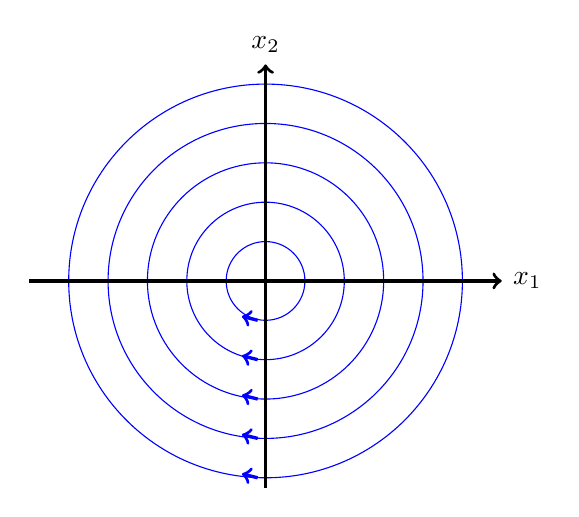
\begin{tikzpicture}
	\draw[color=blue] (0,0) circle(.5);
	\draw[color=blue] (0,0) circle(1);
	\draw[color=blue] (0,0) circle(1.5);
	\draw[color=blue] (0,0) circle(2);
	\draw[color=blue] (0,0) circle(2.5);

	\draw[color=blue,very thick][<-](-.3,-.45)--(-.1,-.5);
	\draw[color=blue,very thick][<-](-.3,-.95)--(-.1,-1);
	\draw[color=blue,very thick][<-](-.3,-1.45)--(-.1,-1.5);
	\draw[color=blue,very thick][<-](-.3,-1.95)--(-.1,-2);
	\draw[color=blue,very thick][<-](-.3,-2.45)--(-.1,-2.5);

	\draw[very thick][->](-3,0)--(3,0) node[right=.2] {$x_1$};
	\draw[very thick][->](0,-2.625)--(0,2.75) node[above=.2] {$x_2$};
\end{tikzpicture}
\hspace*{3cm}
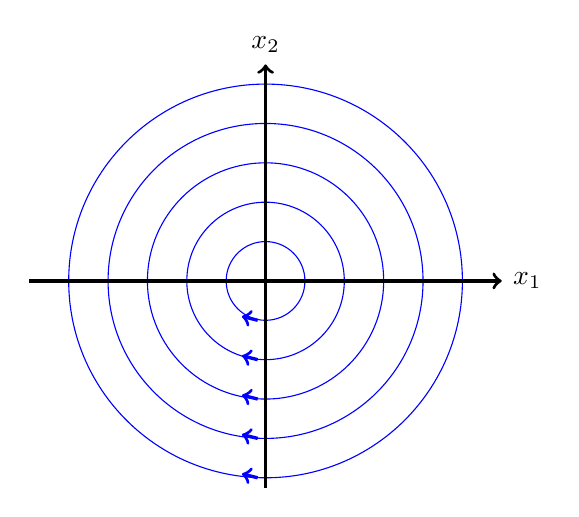
\begin{tikzpicture}
	\draw[color=blue] (0,0) circle(.5);
	\draw[color=blue] (0,0) circle(1);
	\draw[color=blue] (0,0) circle(1.5);
	\draw[color=blue] (0,0) circle(2);
	\draw[color=blue] (0,0) circle(2.5);

	\draw[color=blue,very thick][<-](-.3,-.45)--(-.1,-.5);
	\draw[color=blue,very thick][<-](-.3,-.95)--(-.1,-1);
	\draw[color=blue,very thick][<-](-.3,-1.45)--(-.1,-1.5);
	\draw[color=blue,very thick][<-](-.3,-1.95)--(-.1,-2);
	\draw[color=blue,very thick][<-](-.3,-2.45)--(-.1,-2.5);

	\draw[very thick][->](-3,0)--(3,0) node[right=.2] {$x_1$};
	\draw[very thick][->](0,-2.625)--(0,2.75) node[above=.2] {$x_2$};
\end{tikzpicture}
\end{figure}
Portrety są identyczne. Jedyną różnicą jest szybkość poruszania się trajektorii w dziedzinie czasu. Dla 1 mamy $t$, a dla 2 $10t$



%###################                 2.3.1              #################################%
\pagebreak
\subsection*{Zadanie 2.3.1} {\color{darkgray}
	Podać wartości własne, jakie mogą odpowiadać poniższemu portretowi fazowemu.
\begin{figure}[!h]
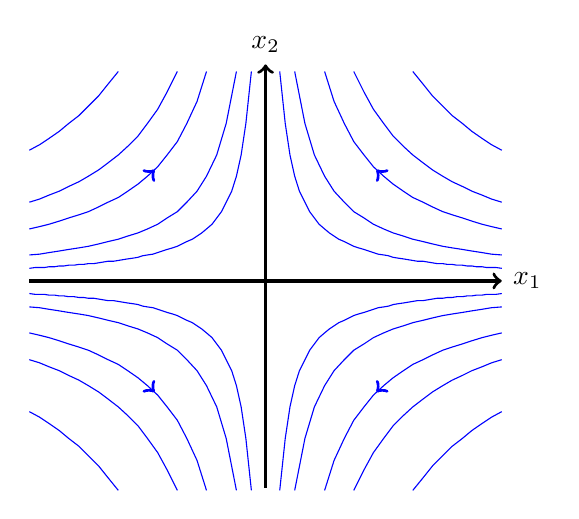
\begin{tikzpicture}
\draw [color=blue](0.18,2.66)--(0.25,2.0)--(0.31,1.6)--(0.37,1.33)--(0.43,1.14)--(0.5,1.0)--(0.56,0.88)--(0.62,0.8)--(0.68,0.72)--(0.75,0.66)--(0.81,0.61)--(0.87,0.57)--(0.93,0.53)--(1.0,0.5)--(1.06,0.47)--(1.12,0.44)--(1.18,0.42)--(1.25,0.4)--(1.31,0.38)--(1.37,0.36)--(1.43,0.34)--(1.5,0.33)--(1.56,0.32)--(1.62,0.3)--(1.68,0.29)--(1.75,0.28)--(1.81,0.27)--(1.87,0.26)--(1.93,0.25)--(2.0,0.25)--(2.06,0.24)--(2.12,0.23)--(2.18,0.22)--(2.25,0.22)--(2.31,0.21)--(2.37,0.21)--(2.43,0.2)--(2.5,0.2)--(2.56,0.19)--(2.62,0.19)--(2.68,0.18)--(2.75,0.18)--(2.81,0.17)--(2.87,0.17)--(2.93,0.17)--(3.0,0.16);
\draw [color=blue](-3.0,-0.16)--(-2.93,-0.17)--(-2.87,-0.17)--(-2.81,-0.17)--(-2.75,-0.18)--(-2.68,-0.18)--(-2.62,-0.19)--(-2.56,-0.19)--(-2.5,-0.2)--(-2.43,-0.2)--(-2.37,-0.21)--(-2.31,-0.21)--(-2.25,-0.22)--(-2.18,-0.22)--(-2.12,-0.23)--(-2.06,-0.24)--(-2.0,-0.25)--(-1.93,-0.25)--(-1.87,-0.26)--(-1.81,-0.27)--(-1.75,-0.28)--(-1.68,-0.29)--(-1.62,-0.3)--(-1.56,-0.32)--(-1.5,-0.33)--(-1.43,-0.34)--(-1.37,-0.36)--(-1.31,-0.38)--(-1.25,-0.4)--(-1.18,-0.42)--(-1.12,-0.44)--(-1.06,-0.47)--(-1.0,-0.5)--(-0.93,-0.53)--(-0.87,-0.57)--(-0.81,-0.61)--(-0.75,-0.66)--(-0.68,-0.72)--(-0.62,-0.8)--(-0.56,-0.88)--(-0.5,-1.0)--(-0.43,-1.14)--(-0.37,-1.33)--(-0.31,-1.6)--(-0.25,-2.0)--(-0.18,-2.66);
\draw [color=blue](0.18,-2.66)--(0.25,-2.0)--(0.31,-1.6)--(0.37,-1.33)--(0.43,-1.14)--(0.5,-1.0)--(0.56,-0.88)--(0.62,-0.8)--(0.68,-0.72)--(0.75,-0.66)--(0.81,-0.61)--(0.87,-0.57)--(0.93,-0.53)--(1.0,-0.5)--(1.06,-0.47)--(1.12,-0.44)--(1.18,-0.42)--(1.25,-0.4)--(1.31,-0.38)--(1.37,-0.36)--(1.43,-0.34)--(1.5,-0.33)--(1.56,-0.32)--(1.62,-0.3)--(1.68,-0.29)--(1.75,-0.28)--(1.81,-0.27)--(1.87,-0.26)--(1.93,-0.25)--(2.0,-0.25)--(2.06,-0.24)--(2.12,-0.23)--(2.18,-0.22)--(2.25,-0.22)--(2.31,-0.21)--(2.37,-0.21)--(2.43,-0.2)--(2.5,-0.2)--(2.56,-0.19)--(2.62,-0.19)--(2.68,-0.18)--(2.75,-0.18)--(2.81,-0.17)--(2.87,-0.17)--(2.93,-0.17)--(3.0,-0.16);
\draw [color=blue](-3.0,0.16)--(-2.93,0.17)--(-2.87,0.17)--(-2.81,0.17)--(-2.75,0.18)--(-2.68,0.18)--(-2.62,0.19)--(-2.56,0.19)--(-2.5,0.2)--(-2.43,0.2)--(-2.37,0.21)--(-2.31,0.21)--(-2.25,0.22)--(-2.18,0.22)--(-2.12,0.23)--(-2.06,0.24)--(-2.0,0.25)--(-1.93,0.25)--(-1.87,0.26)--(-1.81,0.27)--(-1.75,0.28)--(-1.68,0.29)--(-1.62,0.3)--(-1.56,0.32)--(-1.5,0.33)--(-1.43,0.34)--(-1.37,0.36)--(-1.31,0.38)--(-1.25,0.4)--(-1.18,0.42)--(-1.12,0.44)--(-1.06,0.47)--(-1.0,0.5)--(-0.93,0.53)--(-0.87,0.57)--(-0.81,0.61)--(-0.75,0.66)--(-0.68,0.72)--(-0.62,0.8)--(-0.56,0.88)--(-0.5,1.0)--(-0.43,1.14)--(-0.37,1.33)--(-0.31,1.6)--(-0.25,2.0)--(-0.18,2.66);

\draw [color=blue](0.37,2.66)--(0.5,2.0)--(0.62,1.6)--(0.75,1.33)--(0.87,1.14)--(1.0,1.0)--(1.12,0.88)--(1.25,0.8)--(1.37,0.72)--(1.5,0.66)--(1.62,0.61)--(1.75,0.57)--(1.87,0.53)--(2.0,0.5)--(2.12,0.47)--(2.25,0.44)--(2.37,0.42)--(2.5,0.4)--(2.62,0.38)--(2.75,0.36)--(2.87,0.34)--(3.0,0.33);
\draw [color=blue](-3.0,-0.33)--(-2.87,-0.34)--(-2.75,-0.36)--(-2.62,-0.38)--(-2.5,-0.4)--(-2.37,-0.42)--(-2.25,-0.44)--(-2.12,-0.47)--(-2.0,-0.5)--(-1.87,-0.53)--(-1.75,-0.57)--(-1.62,-0.61)--(-1.5,-0.66)--(-1.37,-0.72)--(-1.25,-0.8)--(-1.12,-0.88)--(-1.0,-1.0)--(-0.87,-1.14)--(-0.75,-1.33)--(-0.62,-1.6)--(-0.5,-2.0)--(-0.37,-2.66);
\draw [color=blue](0.37,-2.66)--(0.5,-2.0)--(0.62,-1.6)--(0.75,-1.33)--(0.87,-1.14)--(1.0,-1.0)--(1.12,-0.88)--(1.25,-0.8)--(1.37,-0.72)--(1.5,-0.66)--(1.62,-0.61)--(1.75,-0.57)--(1.87,-0.53)--(2.0,-0.5)--(2.12,-0.47)--(2.25,-0.44)--(2.37,-0.42)--(2.5,-0.4)--(2.62,-0.38)--(2.75,-0.36)--(2.87,-0.34)--(3.0,-0.33);
\draw [color=blue](-3.0,0.33)--(-2.87,0.34)--(-2.75,0.36)--(-2.62,0.38)--(-2.5,0.4)--(-2.37,0.42)--(-2.25,0.44)--(-2.12,0.47)--(-2.0,0.5)--(-1.87,0.53)--(-1.75,0.57)--(-1.62,0.61)--(-1.5,0.66)--(-1.37,0.72)--(-1.25,0.8)--(-1.12,0.88)--(-1.0,1.0)--(-0.87,1.14)--(-0.75,1.33)--(-0.62,1.6)--(-0.5,2.0)--(-0.37,2.66);

\draw [color=blue](0.75,2.66)--(0.87,2.28)--(1.0,2.0)--(1.12,1.77)--(1.25,1.6)--(1.37,1.45)--(1.5,1.33)--(1.62,1.23)--(1.75,1.14)--(1.87,1.06)--(2.0,1.0)--(2.12,0.94)--(2.25,0.88)--(2.37,0.84)--(2.5,0.8)--(2.62,0.76)--(2.75,0.72)--(2.87,0.69)--(3.0,0.66);
\draw [color=blue](-3.0,-0.66)--(-2.87,-0.69)--(-2.75,-0.72)--(-2.62,-0.76)--(-2.5,-0.8)--(-2.37,-0.84)--(-2.25,-0.88)--(-2.12,-0.94)--(-2.0,-1.0)--(-1.87,-1.06)--(-1.75,-1.14)--(-1.62,-1.23)--(-1.5,-1.33)--(-1.37,-1.45)--(-1.25,-1.6)--(-1.12,-1.77)--(-1.0,-2.0)--(-0.87,-2.28)--(-0.75,-2.66);
\draw [color=blue](0.75,-2.66)--(0.87,-2.28)--(1.0,-2.0)--(1.12,-1.77)--(1.25,-1.6)--(1.37,-1.45)--(1.5,-1.33)--(1.62,-1.23)--(1.75,-1.14)--(1.87,-1.06)--(2.0,-1.0)--(2.12,-0.94)--(2.25,-0.88)--(2.37,-0.84)--(2.5,-0.8)--(2.62,-0.76)--(2.75,-0.72)--(2.87,-0.69)--(3.0,-0.66);
\draw [color=blue](-3.0,0.66)--(-2.87,0.69)--(-2.75,0.72)--(-2.62,0.76)--(-2.5,0.8)--(-2.37,0.84)--(-2.25,0.88)--(-2.12,0.94)--(-2.0,1.0)--(-1.87,1.06)--(-1.75,1.14)--(-1.62,1.23)--(-1.5,1.33)--(-1.37,1.45)--(-1.25,1.6)--(-1.12,1.77)--(-1.0,2.0)--(-0.87,2.28)--(-0.75,2.66);

\draw [color=blue](1.12,2.66)--(1.25,2.4)--(1.37,2.18)--(1.5,2.0)--(1.62,1.84)--(1.75,1.71)--(1.87,1.6)--(2.0,1.5)--(2.12,1.41)--(2.25,1.33)--(2.37,1.26)--(2.5,1.2)--(2.62,1.14)--(2.75,1.09)--(2.87,1.04)--(3.0,1.0);
\draw [color=blue](-3.0,-1.0)--(-2.87,-1.04)--(-2.75,-1.09)--(-2.62,-1.14)--(-2.5,-1.2)--(-2.37,-1.26)--(-2.25,-1.33)--(-2.12,-1.41)--(-2.0,-1.5)--(-1.87,-1.6)--(-1.75,-1.71)--(-1.62,-1.84)--(-1.5,-2.0)--(-1.37,-2.18)--(-1.25,-2.4)--(-1.12,-2.66);
\draw [color=blue](1.12,-2.66)--(1.25,-2.4)--(1.37,-2.18)--(1.5,-2.0)--(1.62,-1.84)--(1.75,-1.71)--(1.87,-1.6)--(2.0,-1.5)--(2.12,-1.41)--(2.25,-1.33)--(2.37,-1.26)--(2.5,-1.2)--(2.62,-1.14)--(2.75,-1.09)--(2.87,-1.04)--(3.0,-1.0);
\draw [color=blue](-3.0,1.0)--(-2.87,1.04)--(-2.75,1.09)--(-2.62,1.14)--(-2.5,1.2)--(-2.37,1.26)--(-2.25,1.33)--(-2.12,1.41)--(-2.0,1.5)--(-1.87,1.6)--(-1.75,1.71)--(-1.62,1.84)--(-1.5,2.0)--(-1.37,2.18)--(-1.25,2.4)--(-1.12,2.66);

\draw [color=blue](1.87,2.66)--(2.0,2.5)--(2.12,2.35)--(2.25,2.22)--(2.37,2.1)--(2.5,2.0)--(2.62,1.9)--(2.75,1.81)--(2.87,1.73)--(3.0,1.66);
\draw [color=blue](-3.0,-1.66)--(-2.87,-1.73)--(-2.75,-1.81)--(-2.62,-1.9)--(-2.5,-2.0)--(-2.37,-2.1)--(-2.25,-2.22)--(-2.12,-2.35)--(-2.0,-2.5)--(-1.87,-2.66);
\draw [color=blue](1.87,-2.66)--(2.0,-2.5)--(2.12,-2.35)--(2.25,-2.22)--(2.37,-2.1)--(2.5,-2.0)--(2.62,-1.9)--(2.75,-1.81)--(2.87,-1.73)--(3.0,-1.66);
\draw [color=blue](-3.0,1.66)--(-2.87,1.73)--(-2.75,1.81)--(-2.62,1.9)--(-2.5,2.0)--(-2.37,2.1)--(-2.25,2.22)--(-2.12,2.35)--(-2.0,2.5)--(-1.87,2.66);

	\draw[color=blue,very thick][<-](-1.41,-1.41)--(-1.42,-1.4);
	\draw[color=blue,very thick][<-](-1.41,1.41)--(-1.42,1.4);
	\draw[color=blue,very thick][<-](1.41,1.41)--(1.42,1.4);
	\draw[color=blue,very thick][<-](1.41,-1.41)--(1.42,-1.4);


	\draw[very thick][->](-3,0)--(3,0)node[right=.2] {$x_1$};
	\draw[very thick][->](0,-2.625)--(0,2.75)node[above=.2] {$x_2$};
\end{tikzpicture}
\end{figure}
\\
}\lineh
\\\\
Dla siodła: dwie wartości własne rzeczywiste przeciwnych znaków np 1 i -1\\
$\left[\begin{array}{cc}-1&0\\0&1\end{array}\right]$


%###################                 2.4.1              #################################%
\pagebreak
\subsection*{Zadanie 2.4.1} {\color{darkgray}
	Dla systemu\\
	$\begin{array}{rcl}x(t)+4\ddot{x}(t)+\dot{x}(t)&=&u(t) \\ u(t)&=&k_1\dot{x}(t)-k_2x(t)\end{array}$\\
	zbadać zachowanie się ukłądu w zależności od $k_1$ i $k_2$. Zaznaczyć odpowiednie obszary na płaszczyźnie $k_1 \times k_2$\\
}\lineh
\\\\
$x+4\ddot{x}+\dot{x}=k_1\dot{x}-k_2x$\\
$4\ddot{x}+(1-k_1)\dot{x}+(1+k_2)x=0$\\
wielomian charakterystyczny:\\
$x=e^{\lambda t} \ \ \ \dot{x}=\lambda e^{\lambda t} \ \ \ \ddot{x}=\lambda^2 e^{\lambda t}$\\
$4\lambda^2+(1-k_1)\lambda+1+k_2=0$\\
macierz Hurwitza dla wielomianu stopnia drugiego:
$a_0x^2+a_1x+a_2=0$\\
$\left[\begin{array}{cc}a_1&0\\a_0&a_2\end{array}\right] \ \ $ czyli $\ \ 
\left[\begin{array}{cc}1-k_1&0\\4&1+k_2\end{array}\right]$\\
żeby układ był stabilny to $|a_1|>0$ i $\left|\begin{array}{cc}a_1&0\\a_0&a_2\end{array}\right|>0$\\
więc:\\
$1-k_1>0 \Rightarrow\boxed{ k_1<1}$\\
$(1-k_1)(1+k_2)>0 \Rightarrow 1+k_2>0 \Rightarrow \boxed{k_2>-1}$\\
dla $\Delta<0$ występują oscylacje, więc:\\
$\Delta=(1-k_1)^2-4\cdot4(1-k_2)=(1-k_1)^2-16-16k_2<0$\\
$k_2>\frac{1}{16}(1-k_1)^2-1$\\
\begin{figure}[!h]
\begin{tikzpicture}
\fill[fill=blue, opacity=.2](-6,3)--(1,3)--(1,-1)--(-6,-1);
\draw [pattern=my north east lines, line space=8pt, draw=green!50!black](-6,3)--(-6.0,2.06)--(-5.75,1.84)--(-5.5,1.64)--(-5.25,1.44)--(-5.0,1.25)--(-4.75,1.06)--(-4.5,0.89)--(-4.25,0.72)--(-4.0,0.56)--(-3.75,0.41)--(-3.5,0.26)--(-3.25,0.12)--(-3.0,0.0)--(-2.75,-0.12)--(-2.5,-0.23)--(-2.25,-0.33)--(-2.0,-0.43)--(-1.75,-0.52)--(-1.5,-0.6)--(-1.25,-0.68)--(-1.0,-0.75)--(-0.75,-0.8)--(-0.5,-0.85)--(-0.25,-0.9)--(0.0,-0.93)--(0.25,-0.96)--(0.5,-0.98)--(0.75,-0.99)--(1.0,-1.0)--(1.25,-0.99)--(1.5,-0.98)--(1.75,-0.96)--(2.0,-0.93)--(2.25,-0.9)--(2.5,-0.85)--(2.75,-0.8)--(3.0,-0.75)--(3.25,-0.68)--(3.5,-0.6)--(3.75,-0.52)--(4.0,-0.43)--(4.25,-0.33)--(4.5,-0.23)--(4.75,-0.12)--(5.0,0.0)--(5.25,0.12)--(5.5,0.26)--(5.75,0.41)--(6.0,0.56)--(6,3);
\draw [color=blue](-6.0,2.06)--(-5.75,1.84)--(-5.5,1.64)--(-5.25,1.44)--(-5.0,1.25)--(-4.75,1.06)--(-4.5,0.89)--(-4.25,0.72)--(-4.0,0.56)--(-3.75,0.41)--(-3.5,0.26)--(-3.25,0.12)--(-3.0,0.0)--(-2.75,-0.12)--(-2.5,-0.23)--(-2.25,-0.33)--(-2.0,-0.43)--(-1.75,-0.52)--(-1.5,-0.6)--(-1.25,-0.68)--(-1.0,-0.75)--(-0.75,-0.8)--(-0.5,-0.85)--(-0.25,-0.9)--(0.0,-0.93)--(0.25,-0.96)--(0.5,-0.98)--(0.75,-0.99)--(1.0,-1.0)--(1.25,-0.99)--(1.5,-0.98)--(1.75,-0.96)--(2.0,-0.93)--(2.25,-0.9)--(2.5,-0.85)--(2.75,-0.8)--(3.0,-0.75)--(3.25,-0.68)--(3.5,-0.6)--(3.75,-0.52)--(4.0,-0.43)--(4.25,-0.33)--(4.5,-0.23)--(4.75,-0.12)--(5.0,0.0)--(5.25,0.12)--(5.5,0.26)--(5.75,0.41)--(6.0,0.56);



	\draw[very thick][->](-6,0)--(6,0)node[right=.2] {$k_1$};
	\draw[very thick][->](0,-3)--(0,3)node[above=.2] {$k_2$};

	\draw (-0.1,-1) -- (0.1,-1) node [left=3pt]{{-1}};
	\draw (5,-0.1) -- (5,0.1) node [below=4pt]{{5}};
	\draw (-3,-0.1) -- (-3,0.1) node [below=4pt]{{-3}};
	\draw (1,-0.1) -- (1,0.1) ;
	\node at (1.2,-0.2) {1};

	\draw[dashed, color=red](-6,-1)--(6,-1);
	\draw[dashed, color=red](1,-3)--(1,3);
	\draw[thick](1,-1) circle(.15);
\end{tikzpicture}
\end{figure}
\\
wewnątrz niebieskiego obszaru asymptotycznie stabilny $k_1<1 \wedge k_2>-1)$\\
na czerwonych prostych granicznych stabilny $(k_1=1 \vee k_2=-1)$ bez punktu wspólnego\\
niestabilny na przecięciu prostych i w pozostałych obszarach\\
oscylacje dla zakreskowanego $k_2>\frac{1}{16}(1-k_1)^2-1$



%###################                 2.5.1              #################################%
\pagebreak
\subsection*{Zadanie 2.5.1} {\color{darkgray}
	Zbadać charakter pracy układu\\
	$\begin{array}{rcl}\ddot{x}(t)+\dot{x}(t)+x(t)&=&u(t) \\ u(t)&=&Kx(t)\end{array}$\\
	w zależności od parametru $K$. Zaznaczyć wszystkie istotne rodzaje zachowań na osi liczbowej.\\
}\lineh
\\\\
$\ddot{x}+\dot{x}+x=Kx$\\
$\ddot{x}+\dot{x}+x(1-K)=0$\\
$\lambda^2+\lambda+1-K=0$ wielomian charakterystyczny\\
$\left[\begin{array}{cc}1&0\\1&1-K\end{array}\right]$ macierz Hurwitza\\
$1-K>0 \Rightarrow K<1$\\
$\Delta=1-4(1-K)=-3+4K<0\Rightarrow K<\frac 34$\\
\begin{figure}[!h]
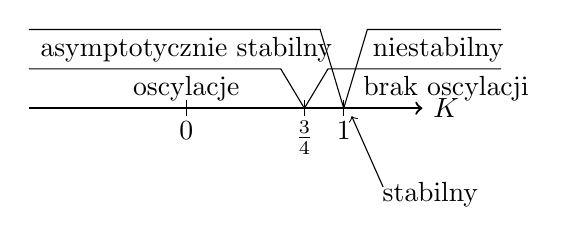
\begin{tikzpicture}
	\draw[thick][->](-2,0)--(3,0)node[right=.2] {$K$};

	\draw (0,-0.1) -- (0,0.1) node [below=4pt]{{0}};
	\draw (2,-0.1) -- (2,0.1) node [below=4pt]{{1}};
	\draw (1.5,-0.1) -- (1.5,0.1) node [below=4pt]{$\frac34$};

	\draw(-2,1)--(1.7,1)--(2,0);
	\node at (0,.75){asymptotycznie stabilny};
	\draw[->](2.5,-1)--(2.1,-0.1);
	\node at (3.1,-1.1){stabilny};
	\draw(4,1)--(2.3,1)--(2,0);
	\node at (3.2,.75){niestabilny};
	\draw(-2,.5)--(1.2,.5)--(1.5,0);
	\node at (0,.25){oscylacje};
	\draw(4,.5)--(1.8,.5)--(1.5,0);
	\node at (3.3,.25){brak oscylacji};

\end{tikzpicture}
\end{figure}
\\

%###################                 2.6.1              #################################%
\pagebreak
\subsection*{Zadanie 2.6.1} {\color{darkgray}
	Dla jakich wartości parametru $k$ system opisany równaniami:\\
	$\begin{array}{rcl}4\dot{x}_1&=&12x_1-0.25kx_2  \\  0.5\dot{x}_2&=&\frac 1kx_1+kx_2\end{array}$\\
	będzie niestabilny.\\
}\lineh
\\\\
$\begin{array}{rcl}\dot{x}_1&=&3x_1-\frac{1}{16}kx_2  \\  \dot{x}_2&=&\frac 2kx_1+2kx_2\end{array}$\\
$\dot{x}=\left[\begin{array}{cc}3&-\frac{1}{16}k\\\frac{2}{k}&2k\end{array}\right]x$\\
$\left|\begin{array}{cc}3-\lambda&-\frac{1}{16}k\\\frac{2}{k}&2k-\lambda\end{array}\right|=(3-\lambda)(2k-\lambda)+(\frac{1}{16}k)(\frac{2}{k})=\lambda^2-(3+2k)\lambda+6k+\frac{1}{8}$ wielomian charakterystyczny\\
$\left[\begin{array}{cc}-(3+2k) &0\\1&6k+\frac 18\end{array}\right]$ macierz Hurwitz'a\\
$-3-2k>0\Rightarrow k<-\frac 32$\\
$-(3+2k)(6k+\frac 18)>0 \Rightarrow 6k+\frac 18>0\Rightarrow k>-\frac 18$\\
stabilny dla $k<-\frac 32 \wedge k>-\frac 18 \Rightarrow k\in \varnothing$\\
niestabilny dla $k \in \mathbb{R}$




%###################                 2.7.1              #################################%
\pagebreak
\subsection*{Zadanie 2.7.1} {\color{darkgray}
	Wyznaczyć macierz $e^{At}$ dla macierzy\\
	$\left[\begin{array}{cc}-2&1\\-2&0\end{array}\right]$\\
}\lineh
\\\\
$e^{At}=P\cdot e^{Jt}\cdot P^{-1}$\\
$e^{Jt}=e^\lambda \cdot J$\\\\
$\left|\begin{array}{cc}-2-\lambda&1\\-2&-\lambda\end{array}\right|=\lambda(2+\lambda)+2=\lambda^2+2\lambda+2=0$\\
$\sqrt{\Delta}=2i$\\
$\lambda_1=\frac{-2+2i}{2}=-1+i \ \ \ \ \ \ \ \lambda_2=-1-i$\\
\\
$\boxed{ \lambda_1=-1+i}$\\
{\color{lightgray}
$\left[\begin{array}{cc}-2+1-i&1\\-2&1-i\end{array}\right]\left[\begin{array}{c}\omega_1\\ \omega_2\end{array}\right]=\left[\begin{array}{c}0\\0\end{array}\right]$\\
$\begin{cases}-(1+i)\omega_i+\omega_2=0 \Rightarrow \omega_2=\omega_1+i\omega_1 \\-2\omega_1+(1-i)\omega_2=0\end{cases}$\\
$-2\omega_1+(1-i)(1+i)\omega_1=0$\\
$-2\omega_1+2\omega_1=0$\\
}
$\boxed{\begin{aligned}
\text{dla }\lambda=a \pm ib\\
J=\left[\begin{array}{cc}a&b\\-b&a\end{array}\right]\\
e^{tJ}=e^{a t}\left[\begin{array}{cc}\cos bt&\sin bt\\-\sin bt& \cos t\end{array}\right]
\end{aligned}}$\\\\
$J=\left[\begin{array}{cc}-1&1\\-1&-1\end{array}\right]$\\
$e^{tJ}=e^{-t}\left[\begin{array}{cc}\cos t & \sin t \\ -\sin t & \cos t\end{array}\right]$\\
$W=\left[\begin{array}{c}1\\1+i\end{array}\right]\omega=s\left[\begin{array}{c}1\\1\end{array}\right]+pi\left[\begin{array}{c}0\\1\end{array}\right]$\\
$P=\left[\begin{array}{cc}1&0\\1&1\end{array}\right]$\\
$P^{-1}=\left[\begin{array}{cc}1&0\\-1&1\end{array}\right]$\\\\
$\boxed{\left[\begin{array}{cc}a&b\\c&d\end{array}\right]^{-1}=\frac{1}{ad-bc}\left[\begin{array}{cc}d&-b\\-c&a\end{array}\right]}$\\\\\\
$e^{At}=\left[\begin{array}{cc}1&0\\1&1\end{array}\right]\cdot e^{-t}\cdot\left[\begin{array}{cc}\cos t&\sin t \\-\sin t &\cos t\end{array}\right]\cdot \left[\begin{array}{cc}1&0\\-1&1\end{array}\right]=e^{-t}\left[\begin{array}{cc}\cos t & \sin t \\ \cos t-\sin t & \sin t +\cos t\end{array}\right]\cdot \left[\begin{array}{cc}1&0\\-1 &1\end{array}\right]=$\\
$=e^{-t}\left[\begin{array}{cc}\cos t - \sin t & \sin t \\-2\sin t &\sin t +\cos t\end{array}\right]$\\


%###################                 2.8.1              #################################%
\pagebreak
\subsection*{Zadanie 2.8.1} {\color{darkgray}
	Wyznaczyć rozwiązanie $x(t), t\geqslant 0$ równania\\
	$\ddot{x}(t)+\dot{x}(t)+3x(t)=0$\\
	$x(0)=1, \ \ \dot{x}(0)=0$\\
}\lineh
\\\\
$x=e^{\lambda t} \ \ \ \dot{x}=\lambda e^{\lambda t} \ \ \ \ddot{x}=\lambda^2 e^{\lambda t}$\\
$\lambda^2e^{\lambda t}+\lambda e^{\lambda t}+3e^{\lambda t}=0$\\
$\lambda^2+\lambda+3=0$\\
$\Delta=1-12=-11<0$\\
$\lambda_1=\alpha+i\beta \ \ \ \ \ \alpha=\frac{-b}{2a} \ \ \ \ \ \alpha=\frac{-1}{2}$\\
$\lambda_2=\alpha-i\beta \ \ \ \ \ \beta=\frac{\sqrt{|\Delta|}}{2a} \ \ \ \ \ \beta=\frac{\sqrt{11}}{2}$\\
\\
$x(t)=Ae^{\alpha t}\cos \beta t+Be^{\alpha t}\sin \beta t$\\
$x(t)=Ae^{-\frac{t}{2}}\cos(\frac{\sqrt{11}}{2}t)+Be^{-\frac t2}\sin(\frac{\sqrt{11}}{2}t)$\\
$x(0)=A\cdot e^0\cdot \cos 0+B\cdot e^0 \cdot  \underbrace{\sin 0}_{=0}=\boxed{A=1}$\\
$\dot{x}(t)=-\beta Ae^{\alpha t}\sin \beta t+\alpha A e^{\alpha t}\cos \beta t+\beta Be^{\alpha t}\cos\beta t+\alpha B e^{\alpha t}\sin \beta t$\\
$\dot{x}(0)=\underbrace{-\frac{\sqrt{11}}{2}\cdot e^0\cdot\sin 0}_{=0}-\frac12\cdot e^0\cos 0+\frac{\sqrt{11}}{2}B\cdot e^0\cdot\cos 0 -\underbrace{\frac12Be^0\sin0}_{=0}=$\\
$=-\frac12+\frac{\sqrt{11}}{2}B=0\Rightarrow\boxed{B=\frac12\cdot\frac{2}{\sqrt{11}}=\frac{\sqrt{11}}{11}}$\\
$\boxed{x(t)=e^{-\frac t2}\cos(\frac{\sqrt{11}}{2}t)+\frac{\sqrt{11}}{11}e^{-\frac t2}\sin(\frac{\sqrt{11}}{2}t)}$\\


%###################                 2.9.1              #################################%
\pagebreak
\subsection*{Zadanie 2.9.1} {\color{darkgray}
	Na gładkim stole leży sznur o długości 0.3 m i masie 50g, przy czym część sznura zwisa ze stołu jak na rysunku. Zamodelować ruch sznura po stole za pomocą równania różniczkowego. Naszkicować portret fazowy systemu opisanego tym równaniem\\}
\begin{figure}[!h]
\begin{tikzpicture}
	
\draw[very thick,pattern=my north east lines, line space=5pt, draw=black] (0,0) -- (4,0) -- (4,-.5) -- (3.2,-.5)--(3.2,-2.5)--(2.7,-2.5)--(2.7,-.5)--(0,-.5);
\filldraw[fill=black] (1,0.05)--(1,.4)--(4,.4)--(4.2,.37)  --(4.3,.3)--(4.37,.2) --(4.4,0)--(4.4,-1.7)--(4.1,-1.7)--(4.1,0.05);

\draw[color=black] (4.1,0)--(5.2,0);
\draw[color=black] (4.1,-1.7)--(5.2,-1.7);
\draw[<->][color=black] (5,0)--(5,-1.7);
\draw[->][color=black] (4.25,-1.7)--(4.25,-2.5);

\node at(5.5,-.9){$x,m$};
\node at(4.3,-2.7){$Q=mg$};
\end{tikzpicture}
\end{figure}
\\
\lineh
\\\\
$l=0.3m \ \ \ m=50g$\\
$m=M\cdot\frac xl$\\
$M\cdot\ddot{x}=m\cdot g$\\
$\cancel{M}\cdot\ddot{x}=\cancel{M}\cdot\frac xl\cdot g$\\
$\ddot{x}=x\frac gl \ \ \ \ k=\frac gl$\\
$x_1=x$\\
$x_2=\dot{x}$\\
$\dot{x}_1=\dot{x}=x_2$\\
$\dot{x}_2=\ddot{x}=x_1k$\\
$\dot{x}=\left[\begin{array}{cc}0&1\\k&0\end{array}\right]x$\\
$\lambda^2-k=0$\\
$\lambda =\pm \sqrt{k}$\\
$J=\left[\begin{array}{cc}\sqrt{k}&0\\0&-\sqrt{k}\end{array}\right]$\\
\\
$\lambda=\sqrt{k}$\\
$\left[\begin{array}{cc}-\sqrt{k}&1\\k&-\sqrt{k}\end{array}\right]\left[\begin{array}{c}\omega_1\\\omega_2\end{array}\right]=\left[\begin{array}{c}0\\0\end{array}\right]$\\
$-\sqrt{k}\omega_1+\omega_2=0$\\
$k\omega_1-\sqrt{k}\omega_2=0$\\
$\omega_2=\sqrt{k}\omega_1$\\
$\left[\begin{array}{c}1\\\sqrt{k}\end{array}\right]$\\
$\left[\begin{array}{cc}0&1\\k&0\end{array}\right]\left[\begin{array}{c}1\\\sqrt{k}\end{array}\right]=\left[\begin{array}{c}\sqrt{k}\\k\end{array}\right]$\\

\begin{figure}[!h]
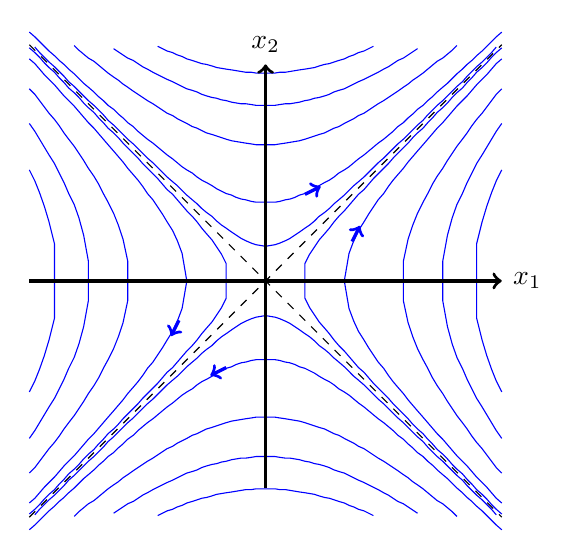
\begin{tikzpicture}
\draw [color=blue](-3.0,2.96)--(-2.93,2.9)--(-2.87,2.84)--(-2.81,2.77)--(-2.75,2.71)--(-2.68,2.65)--(-2.62,2.58)--(-2.56,2.52)--(-2.5,2.45)--(-2.43,2.39)--(-2.37,2.33)--(-2.31,2.26)--(-2.25,2.2)--(-2.18,2.14)--(-2.12,2.07)--(-2.06,2.01)--(-2.0,1.94)--(-1.93,1.88)--(-1.87,1.82)--(-1.81,1.75)--(-1.75,1.69)--(-1.68,1.62)--(-1.62,1.56)--(-1.56,1.49)--(-1.5,1.43)--(-1.43,1.36)--(-1.37,1.3)--(-1.31,1.23)--(-1.25,1.16)--(-1.18,1.1)--(-1.12,1.03)--(-1.06,0.96)--(-1.0,0.89)--(-0.93,0.82)--(-0.87,0.75)--(-0.81,0.67)--(-0.75,0.6)--(-0.68,0.52)--(-0.62,0.43)--(-0.56,0.34)--(-0.5,0.22)--(-0.5,-0.22)--(-0.56,-0.34)--(-0.62,-0.43)--(-0.68,-0.52)--(-0.75,-0.6)--(-0.81,-0.67)--(-0.87,-0.75)--(-0.93,-0.82)--(-1.0,-0.89)--(-1.06,-0.96)--(-1.12,-1.03)--(-1.18,-1.1)--(-1.25,-1.16)--(-1.31,-1.23)--(-1.37,-1.3)--(-1.43,-1.36)--(-1.5,-1.43)--(-1.56,-1.49)--(-1.62,-1.56)--(-1.68,-1.62)--(-1.75,-1.69)--(-1.81,-1.75)--(-1.87,-1.82)--(-1.93,-1.88)--(-2.0,-1.94)--(-2.06,-2.01)--(-2.12,-2.07)--(-2.18,-2.14)--(-2.25,-2.2)--(-2.31,-2.26)--(-2.37,-2.33)--(-2.43,-2.39)--(-2.5,-2.45)--(-2.56,-2.52)--(-2.62,-2.58)--(-2.68,-2.65)--(-2.75,-2.71)--(-2.81,-2.77)--(-2.87,-2.84)--(-2.93,-2.9)--(-3.0,-2.96);
\draw [color=blue](3.0,2.96)--(2.93,2.9)--(2.87,2.84)--(2.81,2.77)--(2.75,2.71)--(2.68,2.65)--(2.62,2.58)--(2.56,2.52)--(2.5,2.45)--(2.43,2.39)--(2.37,2.33)--(2.31,2.26)--(2.25,2.2)--(2.18,2.14)--(2.12,2.07)--(2.06,2.01)--(2.0,1.94)--(1.93,1.88)--(1.87,1.82)--(1.81,1.75)--(1.75,1.69)--(1.68,1.62)--(1.62,1.56)--(1.56,1.49)--(1.5,1.43)--(1.43,1.36)--(1.37,1.3)--(1.31,1.23)--(1.25,1.16)--(1.18,1.1)--(1.12,1.03)--(1.06,0.96)--(1.0,0.89)--(0.93,0.82)--(0.87,0.75)--(0.81,0.67)--(0.75,0.6)--(0.68,0.52)--(0.62,0.43)--(0.56,0.34)--(0.5,0.22)--(0.5,-0.22)--(0.56,-0.34)--(0.62,-0.43)--(0.68,-0.52)--(0.75,-0.6)--(0.81,-0.67)--(0.87,-0.75)--(0.93,-0.82)--(1.0,-0.89)--(1.06,-0.96)--(1.12,-1.03)--(1.18,-1.1)--(1.25,-1.16)--(1.31,-1.23)--(1.37,-1.3)--(1.43,-1.36)--(1.5,-1.43)--(1.56,-1.49)--(1.62,-1.56)--(1.68,-1.62)--(1.75,-1.69)--(1.81,-1.75)--(1.87,-1.82)--(1.93,-1.88)--(2.0,-1.94)--(2.06,-2.01)--(2.12,-2.07)--(2.18,-2.14)--(2.25,-2.2)--(2.31,-2.26)--(2.37,-2.33)--(2.43,-2.39)--(2.5,-2.45)--(2.56,-2.52)--(2.62,-2.58)--(2.68,-2.65)--(2.75,-2.71)--(2.81,-2.77)--(2.87,-2.84)--(2.93,-2.9)--(3.0,-2.96);
\draw [color=blue](-2.93,2.97)--(-2.87,2.9)--(-2.81,2.84)--(-2.75,2.78)--(-2.68,2.72)--(-2.62,2.66)--(-2.56,2.6)--(-2.5,2.53)--(-2.43,2.47)--(-2.37,2.41)--(-2.31,2.35)--(-2.25,2.29)--(-2.18,2.23)--(-2.12,2.17)--(-2.06,2.11)--(-2.0,2.04)--(-1.93,1.98)--(-1.87,1.92)--(-1.81,1.86)--(-1.75,1.8)--(-1.68,1.74)--(-1.62,1.68)--(-1.56,1.62)--(-1.5,1.56)--(-1.43,1.5)--(-1.37,1.44)--(-1.31,1.38)--(-1.25,1.32)--(-1.18,1.26)--(-1.12,1.21)--(-1.06,1.15)--(-1.0,1.09)--(-0.93,1.03)--(-0.87,0.98)--(-0.81,0.92)--(-0.75,0.87)--(-0.68,0.82)--(-0.62,0.76)--(-0.56,0.71)--(-0.5,0.67)--(-0.43,0.62)--(-0.37,0.58)--(-0.31,0.54)--(-0.25,0.51)--(-0.18,0.48)--(-0.12,0.46)--(-0.06,0.45)--(0.0,0.44)--(0.06,0.45)--(0.12,0.46)--(0.18,0.48)--(0.25,0.51)--(0.31,0.54)--(0.37,0.58)--(0.43,0.62)--(0.5,0.67)--(0.56,0.71)--(0.62,0.76)--(0.68,0.82)--(0.75,0.87)--(0.81,0.92)--(0.87,0.98)--(0.93,1.03)--(1.0,1.09)--(1.06,1.15)--(1.12,1.21)--(1.18,1.26)--(1.25,1.32)--(1.31,1.38)--(1.37,1.44)--(1.43,1.5)--(1.5,1.56)--(1.56,1.62)--(1.62,1.68)--(1.68,1.74)--(1.75,1.8)--(1.81,1.86)--(1.87,1.92)--(1.93,1.98)--(2.0,2.04)--(2.06,2.11)--(2.12,2.17)--(2.18,2.23)--(2.25,2.29)--(2.31,2.35)--(2.37,2.41)--(2.43,2.47)--(2.5,2.53)--(2.56,2.6)--(2.62,2.66)--(2.68,2.72)--(2.75,2.78)--(2.81,2.84)--(2.87,2.9)--(2.93,2.97);
\draw [color=blue](-2.93,-2.97)--(-2.87,-2.9)--(-2.81,-2.84)--(-2.75,-2.78)--(-2.68,-2.72)--(-2.62,-2.66)--(-2.56,-2.6)--(-2.5,-2.53)--(-2.43,-2.47)--(-2.37,-2.41)--(-2.31,-2.35)--(-2.25,-2.29)--(-2.18,-2.23)--(-2.12,-2.17)--(-2.06,-2.11)--(-2.0,-2.04)--(-1.93,-1.98)--(-1.87,-1.92)--(-1.81,-1.86)--(-1.75,-1.8)--(-1.68,-1.74)--(-1.62,-1.68)--(-1.56,-1.62)--(-1.5,-1.56)--(-1.43,-1.5)--(-1.37,-1.44)--(-1.31,-1.38)--(-1.25,-1.32)--(-1.18,-1.26)--(-1.12,-1.21)--(-1.06,-1.15)--(-1.0,-1.09)--(-0.93,-1.03)--(-0.87,-0.98)--(-0.81,-0.92)--(-0.75,-0.87)--(-0.68,-0.82)--(-0.62,-0.76)--(-0.56,-0.71)--(-0.5,-0.67)--(-0.43,-0.62)--(-0.37,-0.58)--(-0.31,-0.54)--(-0.25,-0.51)--(-0.18,-0.48)--(-0.12,-0.46)--(-0.06,-0.45)--(0.0,-0.44)--(0.06,-0.45)--(0.12,-0.46)--(0.18,-0.48)--(0.25,-0.51)--(0.31,-0.54)--(0.37,-0.58)--(0.43,-0.62)--(0.5,-0.67)--(0.56,-0.71)--(0.62,-0.76)--(0.68,-0.82)--(0.75,-0.87)--(0.81,-0.92)--(0.87,-0.98)--(0.93,-1.03)--(1.0,-1.09)--(1.06,-1.15)--(1.12,-1.21)--(1.18,-1.26)--(1.25,-1.32)--(1.31,-1.38)--(1.37,-1.44)--(1.43,-1.5)--(1.5,-1.56)--(1.56,-1.62)--(1.62,-1.68)--(1.68,-1.74)--(1.75,-1.8)--(1.81,-1.86)--(1.87,-1.92)--(1.93,-1.98)--(2.0,-2.04)--(2.06,-2.11)--(2.12,-2.17)--(2.18,-2.23)--(2.25,-2.29)--(2.31,-2.35)--(2.37,-2.41)--(2.43,-2.47)--(2.5,-2.53)--(2.56,-2.6)--(2.62,-2.66)--(2.68,-2.72)--(2.75,-2.78)--(2.81,-2.84)--(2.87,-2.9)--(2.93,-2.97);

\draw [color=blue](-3.0,2.82)--(-2.93,2.76)--(-2.87,2.69)--(-2.81,2.62)--(-2.75,2.56)--(-2.68,2.49)--(-2.62,2.42)--(-2.56,2.35)--(-2.5,2.29)--(-2.43,2.22)--(-2.37,2.15)--(-2.31,2.08)--(-2.25,2.01)--(-2.18,1.94)--(-2.12,1.87)--(-2.06,1.8)--(-2.0,1.73)--(-1.93,1.65)--(-1.87,1.58)--(-1.81,1.51)--(-1.75,1.43)--(-1.68,1.35)--(-1.62,1.28)--(-1.56,1.2)--(-1.5,1.11)--(-1.43,1.03)--(-1.37,0.94)--(-1.31,0.85)--(-1.25,0.75)--(-1.18,0.64)--(-1.12,0.51)--(-1.06,0.35)--(-1.0,0.0)--(-0.93,0.0)--(-0.87,0.0)--(-0.81,0.0)--(-0.75,0.0)--(-0.68,0.0)--(-0.62,0.0)--(-0.56,0.0)--(-0.5,0.0)--(-0.43,0.0)--(-0.37,0.0)--(-0.31,0.0)--(-0.25,0.0)--(-0.18,0.0)--(-0.12,0.0)--(-0.06,0.0)--(0.0,0.0)--(0.06,0.0)--(0.12,0.0)--(0.18,0.0)--(0.25,0.0)--(0.31,0.0)--(0.37,0.0)--(0.43,0.0)--(0.5,0.0)--(0.56,0.0)--(0.62,0.0)--(0.68,0.0)--(0.75,0.0)--(0.81,0.0)--(0.87,0.0)--(0.93,0.0)--(1.0,0.0)--(1.06,0.35)--(1.12,0.51)--(1.18,0.64)--(1.25,0.75)--(1.31,0.85)--(1.37,0.94)--(1.43,1.03)--(1.5,1.11)--(1.56,1.2)--(1.62,1.28)--(1.68,1.35)--(1.75,1.43)--(1.81,1.51)--(1.87,1.58)--(1.93,1.65)--(2.0,1.73)--(2.06,1.8)--(2.12,1.87)--(2.18,1.94)--(2.25,2.01)--(2.31,2.08)--(2.37,2.15)--(2.43,2.22)--(2.5,2.29)--(2.56,2.35)--(2.62,2.42)--(2.68,2.49)--(2.75,2.56)--(2.81,2.62)--(2.87,2.69)--(2.93,2.76)--(3.0,2.82);
\draw [color=blue](-3.0,-2.82)--(-2.93,-2.76)--(-2.87,-2.69)--(-2.81,-2.62)--(-2.75,-2.56)--(-2.68,-2.49)--(-2.62,-2.42)--(-2.56,-2.35)--(-2.5,-2.29)--(-2.43,-2.22)--(-2.37,-2.15)--(-2.31,-2.08)--(-2.25,-2.01)--(-2.18,-1.94)--(-2.12,-1.87)--(-2.06,-1.8)--(-2.0,-1.73)--(-1.93,-1.65)--(-1.87,-1.58)--(-1.81,-1.51)--(-1.75,-1.43)--(-1.68,-1.35)--(-1.62,-1.28)--(-1.56,-1.2)--(-1.5,-1.11)--(-1.43,-1.03)--(-1.37,-0.94)--(-1.31,-0.85)--(-1.25,-0.75)--(-1.18,-0.64)--(-1.12,-0.51)--(-1.06,-0.35)--(-1.0,0.0)--(-0.93,0.0)--(-0.87,0.0)--(-0.81,0.0)--(-0.75,0.0)--(-0.68,0.0)--(-0.62,0.0)--(-0.56,0.0)--(-0.5,0.0)--(-0.43,0.0)--(-0.37,0.0)--(-0.31,0.0)--(-0.25,0.0)--(-0.18,0.0)--(-0.12,0.0)--(-0.06,0.0)--(0.0,0.0)--(0.06,0.0)--(0.12,0.0)--(0.18,0.0)--(0.25,0.0)--(0.31,0.0)--(0.37,0.0)--(0.43,0.0)--(0.5,0.0)--(0.56,0.0)--(0.62,0.0)--(0.68,0.0)--(0.75,0.0)--(0.81,0.0)--(0.87,0.0)--(0.93,0.0)--(1.0,0.0)--(1.06,-0.35)--(1.12,-0.51)--(1.18,-0.64)--(1.25,-0.75)--(1.31,-0.85)--(1.37,-0.94)--(1.43,-1.03)--(1.5,-1.11)--(1.56,-1.2)--(1.62,-1.28)--(1.68,-1.35)--(1.75,-1.43)--(1.81,-1.51)--(1.87,-1.58)--(1.93,-1.65)--(2.0,-1.73)--(2.06,-1.8)--(2.12,-1.87)--(2.18,-1.94)--(2.25,-2.01)--(2.31,-2.08)--(2.37,-2.15)--(2.43,-2.22)--(2.5,-2.29)--(2.56,-2.35)--(2.62,-2.42)--(2.68,-2.49)--(2.75,-2.56)--(2.81,-2.62)--(2.87,-2.69)--(2.93,-2.76)--(3.0,-2.82);
\draw [color=blue](-3.0,3.16)--(-2.93,3.1)--(-2.87,3.04)--(-2.81,2.98)--(-2.75,2.92)--(-2.68,2.86)--(-2.62,2.8)--(-2.56,2.75)--(-2.5,2.69)--(-2.43,2.63)--(-2.37,2.57)--(-2.31,2.51)--(-2.25,2.46)--(-2.18,2.4)--(-2.12,2.34)--(-2.06,2.29)--(-2.0,2.23)--(-1.93,2.18)--(-1.87,2.12)--(-1.81,2.07)--(-1.75,2.01)--(-1.68,1.96)--(-1.62,1.9)--(-1.56,1.85)--(-1.5,1.8)--(-1.43,1.75)--(-1.37,1.7)--(-1.31,1.65)--(-1.25,1.6)--(-1.18,1.55)--(-1.12,1.5)--(-1.06,1.45)--(-1.0,1.41)--(-0.93,1.37)--(-0.87,1.32)--(-0.81,1.28)--(-0.75,1.25)--(-0.68,1.21)--(-0.62,1.17)--(-0.56,1.14)--(-0.5,1.11)--(-0.43,1.09)--(-0.37,1.06)--(-0.31,1.04)--(-0.25,1.03)--(-0.18,1.01)--(-0.12,1.0)--(-0.06,1.0)--(0.0,1.0)--(0.06,1.0)--(0.12,1.0)--(0.18,1.01)--(0.25,1.03)--(0.31,1.04)--(0.37,1.06)--(0.43,1.09)--(0.5,1.11)--(0.56,1.14)--(0.62,1.17)--(0.68,1.21)--(0.75,1.25)--(0.81,1.28)--(0.87,1.32)--(0.93,1.37)--(1.0,1.41)--(1.06,1.45)--(1.12,1.5)--(1.18,1.55)--(1.25,1.6)--(1.31,1.65)--(1.37,1.7)--(1.43,1.75)--(1.5,1.8)--(1.56,1.85)--(1.62,1.9)--(1.68,1.96)--(1.75,2.01)--(1.81,2.07)--(1.87,2.12)--(1.93,2.18)--(2.0,2.23)--(2.06,2.29)--(2.12,2.34)--(2.18,2.4)--(2.25,2.46)--(2.31,2.51)--(2.37,2.57)--(2.43,2.63)--(2.5,2.69)--(2.56,2.75)--(2.62,2.8)--(2.68,2.86)--(2.75,2.92)--(2.81,2.98)--(2.87,3.04)--(2.93,3.1)--(3.0,3.16);
\draw [color=blue](-3.0,-3.16)--(-2.93,-3.1)--(-2.87,-3.04)--(-2.81,-2.98)--(-2.75,-2.92)--(-2.68,-2.86)--(-2.62,-2.8)--(-2.56,-2.75)--(-2.5,-2.69)--(-2.43,-2.63)--(-2.37,-2.57)--(-2.31,-2.51)--(-2.25,-2.46)--(-2.18,-2.4)--(-2.12,-2.34)--(-2.06,-2.29)--(-2.0,-2.23)--(-1.93,-2.18)--(-1.87,-2.12)--(-1.81,-2.07)--(-1.75,-2.01)--(-1.68,-1.96)--(-1.62,-1.9)--(-1.56,-1.85)--(-1.5,-1.8)--(-1.43,-1.75)--(-1.37,-1.7)--(-1.31,-1.65)--(-1.25,-1.6)--(-1.18,-1.55)--(-1.12,-1.5)--(-1.06,-1.45)--(-1.0,-1.41)--(-0.93,-1.37)--(-0.87,-1.32)--(-0.81,-1.28)--(-0.75,-1.25)--(-0.68,-1.21)--(-0.62,-1.17)--(-0.56,-1.14)--(-0.5,-1.11)--(-0.43,-1.09)--(-0.37,-1.06)--(-0.31,-1.04)--(-0.25,-1.03)--(-0.18,-1.01)--(-0.12,-1.0)--(-0.06,-1.0)--(0.0,-1.0)--(0.06,-1.0)--(0.12,-1.0)--(0.18,-1.01)--(0.25,-1.03)--(0.31,-1.04)--(0.37,-1.06)--(0.43,-1.09)--(0.5,-1.11)--(0.56,-1.14)--(0.62,-1.17)--(0.68,-1.21)--(0.75,-1.25)--(0.81,-1.28)--(0.87,-1.32)--(0.93,-1.37)--(1.0,-1.41)--(1.06,-1.45)--(1.12,-1.5)--(1.18,-1.55)--(1.25,-1.6)--(1.31,-1.65)--(1.37,-1.7)--(1.43,-1.75)--(1.5,-1.8)--(1.56,-1.85)--(1.62,-1.9)--(1.68,-1.96)--(1.75,-2.01)--(1.81,-2.07)--(1.87,-2.12)--(1.93,-2.18)--(2.0,-2.23)--(2.06,-2.29)--(2.12,-2.34)--(2.18,-2.4)--(2.25,-2.46)--(2.31,-2.51)--(2.37,-2.57)--(2.43,-2.63)--(2.5,-2.69)--(2.56,-2.75)--(2.62,-2.8)--(2.68,-2.86)--(2.75,-2.92)--(2.81,-2.98)--(2.87,-3.04)--(2.93,-3.1)--(3.0,-3.16);

\draw [color=blue](-3.0,2.44)--(-2.93,2.37)--(-2.87,2.29)--(-2.81,2.21)--(-2.75,2.13)--(-2.68,2.05)--(-2.62,1.97)--(-2.56,1.88)--(-2.5,1.8)--(-2.43,1.71)--(-2.37,1.62)--(-2.31,1.53)--(-2.25,1.43)--(-2.18,1.33)--(-2.12,1.23)--(-2.06,1.11)--(-2.0,1.0)--(-1.93,0.86)--(-1.87,0.71)--(-1.81,0.53)--(-1.75,0.25)--(-1.75,-0.25)--(-1.81,-0.53)--(-1.87,-0.71)--(-1.93,-0.86)--(-2.0,-1.0)--(-2.06,-1.11)--(-2.12,-1.23)--(-2.18,-1.33)--(-2.25,-1.43)--(-2.31,-1.53)--(-2.37,-1.62)--(-2.43,-1.71)--(-2.5,-1.8)--(-2.56,-1.88)--(-2.62,-1.97)--(-2.68,-2.05)--(-2.75,-2.13)--(-2.81,-2.21)--(-2.87,-2.29)--(-2.93,-2.37)--(-3.0,-2.44);
\draw [color=blue](3.0,2.44)--(2.93,2.37)--(2.87,2.29)--(2.81,2.21)--(2.75,2.13)--(2.68,2.05)--(2.62,1.97)--(2.56,1.88)--(2.5,1.8)--(2.43,1.71)--(2.37,1.62)--(2.31,1.53)--(2.25,1.43)--(2.18,1.33)--(2.12,1.23)--(2.06,1.11)--(2.0,1.0)--(1.93,0.86)--(1.87,0.71)--(1.81,0.53)--(1.75,0.25)--(1.75,-0.25)--(1.81,-0.53)--(1.87,-0.71)--(1.93,-0.86)--(2.0,-1.0)--(2.06,-1.11)--(2.12,-1.23)--(2.18,-1.33)--(2.25,-1.43)--(2.31,-1.53)--(2.37,-1.62)--(2.43,-1.71)--(2.5,-1.8)--(2.56,-1.88)--(2.62,-1.97)--(2.68,-2.05)--(2.75,-2.13)--(2.81,-2.21)--(2.87,-2.29)--(2.93,-2.37)--(3.0,-2.44);
\draw [color=blue](-2.43,2.99)--(-2.37,2.93)--(-2.31,2.88)--(-2.25,2.83)--(-2.18,2.79)--(-2.12,2.74)--(-2.06,2.69)--(-2.0,2.64)--(-1.93,2.59)--(-1.87,2.55)--(-1.81,2.5)--(-1.75,2.46)--(-1.68,2.41)--(-1.62,2.37)--(-1.56,2.33)--(-1.5,2.29)--(-1.43,2.25)--(-1.37,2.21)--(-1.31,2.17)--(-1.25,2.13)--(-1.18,2.1)--(-1.12,2.06)--(-1.06,2.03)--(-1.0,2.0)--(-0.93,1.96)--(-0.87,1.94)--(-0.81,1.91)--(-0.75,1.88)--(-0.68,1.86)--(-0.62,1.84)--(-0.56,1.82)--(-0.5,1.8)--(-0.43,1.78)--(-0.37,1.77)--(-0.31,1.76)--(-0.25,1.75)--(-0.18,1.74)--(-0.12,1.73)--(-0.06,1.73)--(0.0,1.73)--(0.06,1.73)--(0.12,1.73)--(0.18,1.74)--(0.25,1.75)--(0.31,1.76)--(0.37,1.77)--(0.43,1.78)--(0.5,1.8)--(0.56,1.82)--(0.62,1.84)--(0.68,1.86)--(0.75,1.88)--(0.81,1.91)--(0.87,1.94)--(0.93,1.96)--(1.0,2.0)--(1.06,2.03)--(1.12,2.06)--(1.18,2.1)--(1.25,2.13)--(1.31,2.17)--(1.37,2.21)--(1.43,2.25)--(1.5,2.29)--(1.56,2.33)--(1.62,2.37)--(1.68,2.41)--(1.75,2.46)--(1.81,2.5)--(1.87,2.55)--(1.93,2.59)--(2.0,2.64)--(2.06,2.69)--(2.12,2.74)--(2.18,2.79)--(2.25,2.83)--(2.31,2.88)--(2.37,2.93)--(2.43,2.99);
\draw [color=blue](-2.43,-2.99)--(-2.37,-2.93)--(-2.31,-2.88)--(-2.25,-2.83)--(-2.18,-2.79)--(-2.12,-2.74)--(-2.06,-2.69)--(-2.0,-2.64)--(-1.93,-2.59)--(-1.87,-2.55)--(-1.81,-2.5)--(-1.75,-2.46)--(-1.68,-2.41)--(-1.62,-2.37)--(-1.56,-2.33)--(-1.5,-2.29)--(-1.43,-2.25)--(-1.37,-2.21)--(-1.31,-2.17)--(-1.25,-2.13)--(-1.18,-2.1)--(-1.12,-2.06)--(-1.06,-2.03)--(-1.0,-2.0)--(-0.93,-1.96)--(-0.87,-1.94)--(-0.81,-1.91)--(-0.75,-1.88)--(-0.68,-1.86)--(-0.62,-1.84)--(-0.56,-1.82)--(-0.5,-1.8)--(-0.43,-1.78)--(-0.37,-1.77)--(-0.31,-1.76)--(-0.25,-1.75)--(-0.18,-1.74)--(-0.12,-1.73)--(-0.06,-1.73)--(0.0,-1.73)--(0.06,-1.73)--(0.12,-1.73)--(0.18,-1.74)--(0.25,-1.75)--(0.31,-1.76)--(0.37,-1.77)--(0.43,-1.78)--(0.5,-1.8)--(0.56,-1.82)--(0.62,-1.84)--(0.68,-1.86)--(0.75,-1.88)--(0.81,-1.91)--(0.87,-1.94)--(0.93,-1.96)--(1.0,-2.0)--(1.06,-2.03)--(1.12,-2.06)--(1.18,-2.1)--(1.25,-2.13)--(1.31,-2.17)--(1.37,-2.21)--(1.43,-2.25)--(1.5,-2.29)--(1.56,-2.33)--(1.62,-2.37)--(1.68,-2.41)--(1.75,-2.46)--(1.81,-2.5)--(1.87,-2.55)--(1.93,-2.59)--(2.0,-2.64)--(2.06,-2.69)--(2.12,-2.74)--(2.18,-2.79)--(2.25,-2.83)--(2.31,-2.88)--(2.37,-2.93)--(2.43,-2.99);


\draw [color=blue](-3.0,2.0)--(-2.93,1.9)--(-2.87,1.8)--(-2.81,1.7)--(-2.75,1.6)--(-2.68,1.49)--(-2.62,1.37)--(-2.56,1.25)--(-2.5,1.11)--(-2.43,0.97)--(-2.37,0.8)--(-2.31,0.58)--(-2.25,0.25)--(-2.25,-0.25)--(-2.31,-0.58)--(-2.37,-0.8)--(-2.43,-0.97)--(-2.5,-1.11)--(-2.56,-1.25)--(-2.62,-1.37)--(-2.68,-1.49)--(-2.75,-1.6)--(-2.81,-1.7)--(-2.87,-1.8)--(-2.93,-1.9)--(-3.0,-2.0);
\draw [color=blue](3.0,2.0)--(2.93,1.9)--(2.87,1.8)--(2.81,1.7)--(2.75,1.6)--(2.68,1.49)--(2.62,1.37)--(2.56,1.25)--(2.5,1.11)--(2.43,0.97)--(2.37,0.8)--(2.31,0.58)--(2.25,0.25)--(2.25,-0.25)--(2.31,-0.58)--(2.37,-0.8)--(2.43,-0.97)--(2.5,-1.11)--(2.56,-1.25)--(2.62,-1.37)--(2.68,-1.49)--(2.75,-1.6)--(2.81,-1.7)--(2.87,-1.8)--(2.93,-1.9)--(3.0,-2.0);
\draw [color=blue](-1.93,2.95)--(-1.87,2.91)--(-1.81,2.87)--(-1.75,2.83)--(-1.68,2.8)--(-1.62,2.76)--(-1.56,2.72)--(-1.5,2.69)--(-1.43,2.65)--(-1.37,2.62)--(-1.31,2.59)--(-1.25,2.56)--(-1.18,2.53)--(-1.12,2.5)--(-1.06,2.47)--(-1.0,2.44)--(-0.93,2.42)--(-0.87,2.4)--(-0.81,2.37)--(-0.75,2.35)--(-0.68,2.33)--(-0.62,2.32)--(-0.56,2.3)--(-0.5,2.29)--(-0.43,2.27)--(-0.37,2.26)--(-0.31,2.25)--(-0.25,2.25)--(-0.18,2.24)--(-0.12,2.23)--(-0.06,2.23)--(0.0,2.23)--(0.06,2.23)--(0.12,2.23)--(0.18,2.24)--(0.25,2.25)--(0.31,2.25)--(0.37,2.26)--(0.43,2.27)--(0.5,2.29)--(0.56,2.3)--(0.62,2.32)--(0.68,2.33)--(0.75,2.35)--(0.81,2.37)--(0.87,2.4)--(0.93,2.42)--(1.0,2.44)--(1.06,2.47)--(1.12,2.5)--(1.18,2.53)--(1.25,2.56)--(1.31,2.59)--(1.37,2.62)--(1.43,2.65)--(1.5,2.69)--(1.56,2.72)--(1.62,2.76)--(1.68,2.8)--(1.75,2.83)--(1.81,2.87)--(1.87,2.91)--(1.93,2.95);
\draw [color=blue](-1.93,-2.95)--(-1.87,-2.91)--(-1.81,-2.87)--(-1.75,-2.83)--(-1.68,-2.8)--(-1.62,-2.76)--(-1.56,-2.72)--(-1.5,-2.69)--(-1.43,-2.65)--(-1.37,-2.62)--(-1.31,-2.59)--(-1.25,-2.56)--(-1.18,-2.53)--(-1.12,-2.5)--(-1.06,-2.47)--(-1.0,-2.44)--(-0.93,-2.42)--(-0.87,-2.4)--(-0.81,-2.37)--(-0.75,-2.35)--(-0.68,-2.33)--(-0.62,-2.32)--(-0.56,-2.3)--(-0.5,-2.29)--(-0.43,-2.27)--(-0.37,-2.26)--(-0.31,-2.25)--(-0.25,-2.25)--(-0.18,-2.24)--(-0.12,-2.23)--(-0.06,-2.23)--(0.0,-2.23)--(0.06,-2.23)--(0.12,-2.23)--(0.18,-2.24)--(0.25,-2.25)--(0.31,-2.25)--(0.37,-2.26)--(0.43,-2.27)--(0.5,-2.29)--(0.56,-2.3)--(0.62,-2.32)--(0.68,-2.33)--(0.75,-2.35)--(0.81,-2.37)--(0.87,-2.4)--(0.93,-2.42)--(1.0,-2.44)--(1.06,-2.47)--(1.12,-2.5)--(1.18,-2.53)--(1.25,-2.56)--(1.31,-2.59)--(1.37,-2.62)--(1.43,-2.65)--(1.5,-2.69)--(1.56,-2.72)--(1.62,-2.76)--(1.68,-2.8)--(1.75,-2.83)--(1.81,-2.87)--(1.87,-2.91)--(1.93,-2.95);

\draw [color=blue](-3.0,1.41)--(-2.93,1.27)--(-2.87,1.12)--(-2.81,0.95)--(-2.75,0.75)--(-2.68,0.47)--(-2.68,-0.47)--(-2.75,-0.75)--(-2.81,-0.95)--(-2.87,-1.12)--(-2.93,-1.27)--(-3.0,-1.41);
\draw [color=blue](3.0,1.41)--(2.93,1.27)--(2.87,1.12)--(2.81,0.95)--(2.75,0.75)--(2.68,0.47)--(2.68,-0.47)--(2.75,-0.75)--(2.81,-0.95)--(2.87,-1.12)--(2.93,-1.27)--(3.0,-1.41);
\draw [color=blue](-1.37,2.98)--(-1.31,2.95)--(-1.25,2.92)--(-1.18,2.9)--(-1.12,2.87)--(-1.06,2.85)--(-1.0,2.82)--(-0.93,2.8)--(-0.87,2.78)--(-0.81,2.76)--(-0.75,2.75)--(-0.68,2.73)--(-0.62,2.71)--(-0.56,2.7)--(-0.5,2.69)--(-0.43,2.68)--(-0.37,2.67)--(-0.31,2.66)--(-0.25,2.65)--(-0.18,2.65)--(-0.12,2.64)--(-0.06,2.64)--(0.0,2.64)--(0.06,2.64)--(0.12,2.64)--(0.18,2.65)--(0.25,2.65)--(0.31,2.66)--(0.37,2.67)--(0.43,2.68)--(0.5,2.69)--(0.56,2.7)--(0.62,2.71)--(0.68,2.73)--(0.75,2.75)--(0.81,2.76)--(0.87,2.78)--(0.93,2.8)--(1.0,2.82)--(1.06,2.85)--(1.12,2.87)--(1.18,2.9)--(1.25,2.92)--(1.31,2.95)--(1.37,2.98);
\draw [color=blue](-1.37,-2.98)--(-1.31,-2.95)--(-1.25,-2.92)--(-1.18,-2.9)--(-1.12,-2.87)--(-1.06,-2.85)--(-1.0,-2.82)--(-0.93,-2.8)--(-0.87,-2.78)--(-0.81,-2.76)--(-0.75,-2.75)--(-0.68,-2.73)--(-0.62,-2.71)--(-0.56,-2.7)--(-0.5,-2.69)--(-0.43,-2.68)--(-0.37,-2.67)--(-0.31,-2.66)--(-0.25,-2.65)--(-0.18,-2.65)--(-0.12,-2.64)--(-0.06,-2.64)--(0.0,-2.64)--(0.06,-2.64)--(0.12,-2.64)--(0.18,-2.65)--(0.25,-2.65)--(0.31,-2.66)--(0.37,-2.67)--(0.43,-2.68)--(0.5,-2.69)--(0.56,-2.7)--(0.62,-2.71)--(0.68,-2.73)--(0.75,-2.75)--(0.81,-2.76)--(0.87,-2.78)--(0.93,-2.8)--(1.0,-2.82)--(1.06,-2.85)--(1.12,-2.87)--(1.18,-2.9)--(1.25,-2.92)--(1.31,-2.95)--(1.37,-2.98);


	\draw[color=blue,very thick][<-](-.7,-1.2)--(-.5,-1.1);
	\draw[color=blue,very thick][<-](.7,1.2)--(.5,1.1);
	\draw[color=blue,very thick][<-](1.2,.7)--(1.1,.5);
	\draw[color=blue,very thick][<-](-1.2,-.7)--(-1.1,-.5);

	\draw[dashed](-3,-3)--(3,3);
	\draw[dashed](-3,3)--(3,-3);

	\draw[very thick][->](-3,0)--(3,0) node[right=.2] {$x_1$};
	\draw[very thick][->](0,-2.625)--(0,2.75) node[above=.2] {$x_2$};
\end{tikzpicture}
\end{figure}



%###################                 2.10.1              #################################%
\pagebreak
\subsection*{Zadanie 2.10.1} {\color{darkgray}
	Dany jest system opisany równaniem\\
	$\dot{x}_1(t)=-\pi x_2(t)$\\
	$\dot{x}_2(t)=\pi x_1(t)$\\
	Naszkicować zbiór punktów powstałych z trajektorii stanu systemu w chwili $t=0.75s$ dla warunków początkowych branych ze zbioru $X=\{(x_1,x_2)\in \mathbb{R}^2:|x_1+x_2|=1\}$\\
}\lineh
\\\\
$\dot{x}=\left[\begin{array}{cc}0&-\pi\\\pi&0\end{array}\right]x$\\
$\left|\begin{array}{cc}-\lambda&-\pi\\\pi&-\lambda\end{array}\right|=\lambda^2+\pi^2=0\Rightarrow\lambda^2=-\pi^2 \ \ \ \ \ \ \ \lambda=\pm i\pi$\\
$J=\left[\begin{array}{cc}0&-\pi\\\pi&0\end{array}\right]$\\
$A = J$, $a=0, b=\pi$\\
$e^{tJ}=e^{t}\left[\begin{array}{cc}\cos(\pi t)&\sin(\pi t)\\-\sin(\pi t)&\cos(\pi t)\end{array}\right]$\\
$x(t)=e^{tJ}x(0)+\underbrace{\int_0^te^{(t-\tau)A}Bu(\tau)\ d\tau}_{=0 \text{, \ bo }u=0 \ \ B=0}$\\
$x(t)=e^{tJ}x(0)$\\\\
$x(t)=\left[\begin{array}{cc}\cos(\pi t)&\sin(\pi t)\\-\sin(\pi t)&\cos(\pi t)\end{array}\right]x(0)$\\
$t=\frac 34 s$\\
$x(\frac 34)=\left[\begin{array}{cc}-\frac{\sqrt{2}}{2}&\frac{\sqrt{2}}{2}\\-\frac{\sqrt{2}}{2}&-\frac{\sqrt{2}}{2}\end{array}\right]x(0)=-\frac{\sqrt{2}}{2}\left[\begin{array}{cc}1&-1\\1&1\end{array}\right]x(0)$\\
$\begin{cases}
x_1(\frac34)=-\frac{\sqrt{2}}{2}(x_1(0)-x_2(0))\\
x_2(\frac34)=-\frac{\sqrt{2}}{2}(x_1(0)+x_2(0))\\
|x_1+x_2|=1\Rightarrow \begin{array}{ccc}x_1+x_2=1&\vee&x_1+x_2=-1 \\ x_1=1-x_2&\vee& x_1=-1-x_2\end{array}
\end{cases}$\\
$\begin{cases}
x_1(\frac34)=-\frac{\sqrt{2}}{2}(-x_2(0)+1-x_2(0))=-\frac{\sqrt{2}}{2}-\sqrt{2}x_2(0)\\
x_2(\frac34)=-\frac{\sqrt{2}}{2}(-x_2(0)+1+x_2(0))=-\frac{\sqrt{2}}{2}
\end{cases}$\\
$\begin{cases}
x_1(\frac34)=-\frac{\sqrt{2}}{2}(-1-x_2(0)-x_2(0))=\frac{\sqrt{2}}{2}+\sqrt{2}x_2(0)\\
x_2(\frac34)=-\frac{\sqrt{2}}{2}(-1-x_2(0)+x_2(0))=\frac{\sqrt{2}}{2}
\end{cases}$\\

\begin{figure}[!h]
\begin{tikzpicture}
	\draw [color=blue](-3,1)--(3,1);
	\draw [color=blue](-3,-1)--(3,-1);


	\draw[very thick][->](-3,0)--(3,0) node[right=.2] {$x_1(\frac34)$};
	\draw[very thick][->](0,-2.625)--(0,2.75) node[above=.2] {$x_2(\frac34)$};
\end{tikzpicture}
\end{figure}


%  \left[\begin{array}{cc}\end{array}\right]